% -----------------------------------------------
% SMC 2026 version of "Acoustic Overspecification in EDM Taxonomy"
% Converted from ICASSP 2026 format
% -----------------------------------------------
\documentclass{article}
\usepackage{smc2026}
\usepackage[caption=false, font=footnotesize]{subfig}
\usepackage{paralist}
\usepackage[figure,table]{hypcap}
\usepackage[english]{babel}
\usepackage{amsmath}
\usepackage{booktabs}
\usepackage{multirow}

% Title.
\def\papertitle{Acoustic Overspecification \\\ in Electronic Dance Music Taxonomy}

% Authors (SMC is single-blind, names visible)
\author[1]{\mbox{\firstname{Weilun}\lastname{Xu}}}
\author[1]{\mbox{\firstname{Tianhao}\lastname{Dai}}}
\author[1]{\mbox{\firstname{Oscar}\lastname{Goudet}}}
\author[2]{\mbox{\firstname{Xiaoxuan}\lastname{Wang}}}

%Affiliations
\affil[1]{\department{School of Computer and Communication Sciences (IC)}\institution{École Polytechnique Fédérale de Lausanne}\country{Switzerland}\affiliationtype{University}}
\affil[2]{\department{Digital and Cognitive Musicology Lab}\institution{École Polytechnique Fédérale de Lausanne}\country{Switzerland}\affiliationtype{University}}

% Complete setup stage
\completesetup

% Title.
\title{\papertitle}

\begin{document}
	%
	\capstartfalse
	\maketitle
	\capstarttrue
	%

	\begin{abstract}
		Electronic Dance Music (EDM) classification typically relies on industry-defined taxonomies, with current supervised approaches naturally assuming the validity of prescribed subgenre labels. However, whether these commercial distinctions reflect genuine acoustic differences remains largely unexplored. In this paper, we propose an unsupervised approach to discover the natural acoustic structure of EDM independent of commercial labels. To address the historical lack of EDM-specific feature design in MIR, we systematically construct a tailored acoustic feature space capturing the genre's defining production techniques, spectral textures, and layered rhythmic patterns. To ensure our findings reflect inherent acoustic structure rather than feature engineering artifacts, we validate our clustering against state-of-the-art pre-trained audio embeddings (MERT and CLAP). Across both our bespoke feature space and the pre-trained embeddings, clustering converges to 19--23 natural acoustic families---far fewer than the prescribed 35. This provides consistent evidence that the current commercial EDM taxonomy is acoustically overspecified by over one-third.
	\end{abstract}

	\section{Introduction}\label{sec:intro}
	Electronic Dance Music (EDM) presents unique challenges for genre classification. Commercial platforms like Beatport\footnote{\url{https://www.beatport.com} -- leading digital music platform specializing in electronic dance music.} categorize tracks into 35 or more distinct subgenres, yet whether these distinctions reflect genuine acoustic differences or primarily serve commercial and cultural functions remains an open question~\cite{brackett2016}. To understand this tension, we distinguish between two fundamentally different conceptions of genre. \emph{Acoustic genres} are computationally discoverable clusters based on measurable sonic features---tempo, timbre, harmonic content, and rhythmic patterns---reflecting genuine perceptual differences. \emph{Cultural genres}, by contrast, are socially constructed categories that serve marketing differentiation, regional scene identity, and what Thornton terms ``subcultural capital''---knowledge of micro-genres functioning as cultural currency within dance music communities~\cite{thornton2013club}. EDM genres thus operate less as stable taxonomic categories and more as what Thornton describes as ``taste cultures'': fluid social formations organized around aesthetic preferences and production techniques.

	Previous EDM classification research has predominantly employed supervised learning with industry-provided labels~\cite{caparrini2020,shu2024,knees2015,faraldo2016,popli2022,hsu2021}. However, these approaches assume label validity without examining whether the prescribed taxonomy aligns with acoustic reality. This assumption is problematic: genre distinctions in EDM are frequently tied to specific production tools and techniques---from the Roland TB-303 that defined Acid House to the sidechain-compression aesthetics of modern Progressive House~\cite{butler2014playing}---and these production-level cues may not be fully captured by standard audio features, further complicating the relationship between acoustic measurement and genre identity.

	\begin{figure}[t]
		\centering
		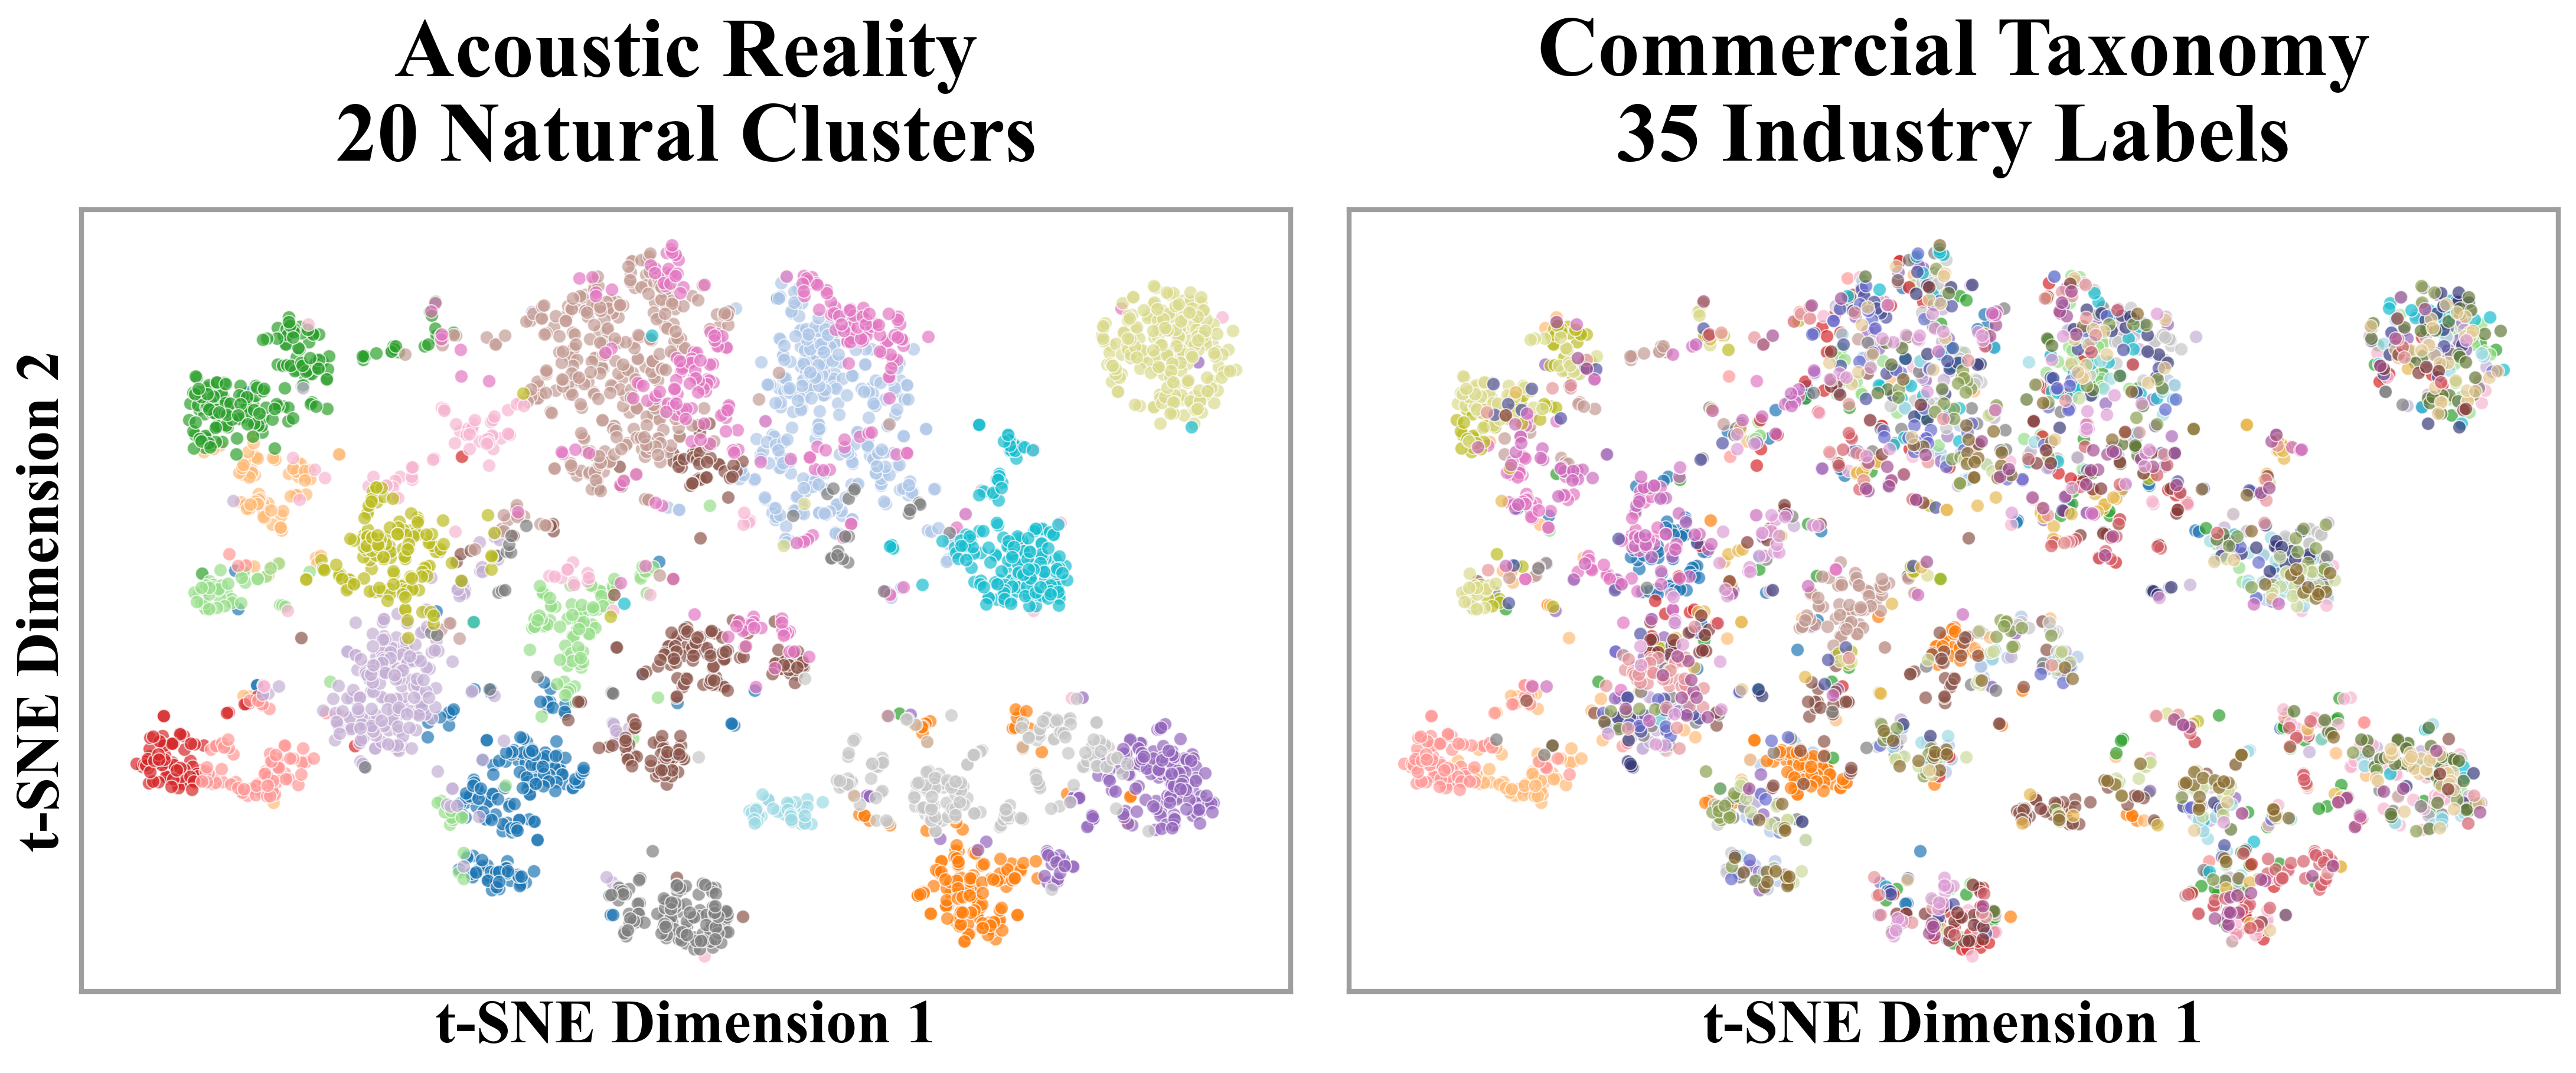
\includegraphics[width=\columnwidth]{figs/paper/fig1_tsne.png}
		\caption{t-SNE projection of selected acoustic features (Section~\ref{ssec:features}). Left: 20 natural clusters discovered via K-means optimization. Right: identical projection colored by the 35 commercial Beatport genre labels. The severe color fragmentation within spatially cohesive acoustic regions visually demonstrates the overspecification of the commercial taxonomy.}
		\label{fig:tsne}
	\end{figure}

	This structural misalignment motivates our central research question: Does EDM's commercial genre taxonomy reflect its underlying acoustic structure? Figure~\ref{fig:tsne} visualizes this tension---when the same tracks are organized by acoustic similarity versus market labels, different patterns emerge. We investigate this disconnect through clustering, allowing natural groupings to emerge without presupposing the validity of industry categories.

	Our contributions include: (1) A bespoke acoustic feature space tailored to EDM---spanning spectral-harmonic, production, texture, and rhythmic dimensions---applicable to further downstream tasks such as genre discovery, recommendation, and playlist generation, (2) Evidence that EDM's commercial taxonomy is overspecified by over one-third: convergence to $\sim$20 natural clusters versus 35 prescribed genres across diverse feature representations and clustering methods.


	\section{Dataset and Features}\label{sec:data}
	
	\subsection{Dataset}\label{ssec:dataset}
	We construct our dataset from Beatport, collecting the top 100 hit tracks from each of 35 genres (3,500 total) as of March 2025. On Beatport, genre labels are assigned by artists and labels who select from a curated taxonomy maintained by the platform; genres thus originate from community and artist practice but are mediated through Beatport's fixed category list. Each track is listed under a single primary genre, so our dataset contains no duplicate tracks across categories. While broader terms like ``Techno'' qualify multiple Beatport categories (e.g., Hard Techno, Melodic House \& Techno), we treat each strictly as a distinct genre. One category, DJ Tools, is not a traditional genre but a utility class containing loops, samples, and mixing elements; we retain it because it is part of Beatport's official taxonomy, and a sensitivity analysis (Appendix~\ref{app:sensitivity}) confirms its inclusion does not materially affect our results. We extract 2-minute previews at 320\,kbps with metadata including BPM, key, length, and genre labels. These chart-topping tracks represent established genre exemplars validated by commercial success.

	\subsection{Feature Extraction}\label{ssec:features}
	We extract 194 acoustic dimensions per track, processing audio identically at 44.1\,kHz. To capture EDM's production techniques, texture, and layered rhythmic patterns, we extract three complementary feature groups (see Appendix~\ref{app:features} and Table~\ref{tab:feature_taxonomy} for a complete taxonomy).

	\textbf{Conventional MIR Features} (92 dimensions): Following established baselines~\cite{caparrini2020}, we extract (1) spectral shape features including centroid, spread, entropy, flux, and rolloff, (2) timbral descriptors comprising 13-band MFCCs, (3) harmonic features via 12-dimensional chroma vectors, and (4) rhythmic measures including autocorrelation-derived danceability, beat histogram periodicity, and frequency-band beat emphasis (energy restricted to beat-frames across 6 octave-spaced bands). We compute the mean and standard deviation of these frame-level metrics.
	
	\textbf{EDM Production Features} (38 dimensions): We adapt standard audio analysis tools alongside novel proxies to capture club-oriented mixing aesthetics. For dynamics, we compute the Harmonic-to-Percussive (H/P) energy ratio, crest factor, and RMS kurtosis using median-filtering separated components~\cite{fitzgerald2010} to quantify drum prominence and dynamic range compression (brickwalling). For spectral texture, we extract 7-band spectral contrast~\cite{jiang2002} to track synthesizer sharpness versus noise. For bass design, we introduce a novel sub-bass ratio (power beneath 60\,Hz) and a sidechain pumping proxy that measures the negative correlation between the kick-band envelope and high-frequency synthesizer envelope.

	\textbf{Tempogram-based Features} (64 dimensions): Standard tempo estimation fails to capture EDM's layered rhythmic structures. Following~\cite{grosche2012}, we compute three complementary tempogram representations. The Fourier tempogram applies the short-time Fourier transform to a novelty curve (onset-strength envelope) and converts the result to tempo units:
	\begin{equation}
		T^F(t,\tau) = |\mathcal{F}(t,\tau/60)|
	\end{equation}
	where $t$ is the time frame, $\tau$ is tempo in BPM, and $\mathcal{F}(t,\omega)$ denotes the windowed Fourier transform of the novelty curve at frequency $\omega$. The autocorrelation tempogram similarly captures subharmonic periodicities via local autocorrelation. To remove octave ambiguities in both representations, we derive cyclic tempograms by pooling all tempi related by powers of two into a single octave:
	\begin{equation}
		C_\rho(t,s) = \sum_{\lambda \in [s\cdot\rho]} T(t,\lambda), \quad s \in [1,2)
	\end{equation}
	where $T(t,\lambda)$ is the tempogram value at time $t$ and tempo $\lambda$, $\rho$ is a reference tempo (60\,BPM), $s$ indexes position within the octave, and the sum runs over all $\lambda$ in the equivalence class $[s\cdot\rho]$ (i.e., tempi differing by powers of two). From each representation, we extract statistical summaries of the top tempo bins, including their BPM, mean magnitude, and temporal variability.

	To isolate EDM's inherent acoustic organization from potential feature engineering artifacts, we additionally extract embeddings from two state-of-the-art pre-trained models:

	\textbf{MERT-95M} (768 dimensions): a music-specific transformer trained on 160M music clips using masked language modeling~\cite{li2024mert}. MERT learns hierarchical music representations without genre labels. \textbf{CLAP-tiny} (512 dimensions): a contrastive audio-language model trained on 630K audio-text pairs~\cite{wu2023clap}. CLAP's multimodal training provides a domain-agnostic perspective.

	These embeddings serve as independent validation: if diverse feature representations converge to similar natural cluster counts despite different architectures, training objectives, and dimensionalities, this provides strong evidence that our discovered taxonomy reflects EDM's inherent acoustic organization rather than methodological choices.


	\subsection{Feature Engineering and Selection}\label{ssec:selection}

	We apply multi-scale preprocessing to enrich the feature space: polynomial expansion (degree-2 interaction terms between features), log-transformation of skewed distributions, and cross-domain products (e.g., spectral $\times$ rhythmic). To stabilize variance and address the severe skewness of many acoustic features, we apply a Yeo--Johnson Power Transformation~\cite{yeo2000new} to approximate Gaussian distributions, optimizing the space for variance-based clustering algorithms like K-Means.

	The expanded feature space (395 features) contains substantial redundancy, so we apply a two-stage selection pipeline. First, we remove correlated features (Pearson $|r| > 0.95$), reducing the set to 181. Second, we apply \emph{hybrid selection} combining two complementary objectives:

	\textbf{Stage 1: Greedy silhouette-optimized selection.} Starting from the single feature with the highest silhouette score (K-means, $k$=35, 50 restarts), we iteratively add the feature that maximizes silhouette when combined with the current set. This yields 20 features optimized for internal cluster quality.

	\textbf{Stage 2: Ensemble genre-discriminative top-up.} We compute a multi-criteria ensemble score
	\begin{equation}
		S_{\mathrm{ens}}(f_i) = \frac{1}{|M|}\sum_{m \in M} w_m \cdot \hat{S}_m(f_i)
	\end{equation}
	where $\hat{S}_m(f_i) \in [0,1]$ is the min-max normalized importance score from method $m$, and $M$ includes ANOVA F-statistic, mutual information, Random Forest importance, Extra Trees importance, variance-based scoring, and cluster separation score ($|M|=6$, equal weights $w_m=1$). The 5 highest-scoring features not already selected in Stage~1 are added, yielding a final set of 25 features that balance cluster separability with genre-discriminative diversity.


	\section{Methods}\label{sec:method}
	\subsection{Clustering Methods}
	We employ two clustering paradigms: divisive hierarchical clustering provides a top-down partitioning approach, while K-means serves as a highly robust, centroid-based optimization.

	\textbf{Hierarchical Divisive Clustering.} We implement a divisive hierarchical clustering algorithm that iteratively splits clusters based on a heterogeneity score:
	\begin{equation}
		H(C) = \sigma^2(C) \cdot (1 + \text{sil}(C)) \cdot \log(|C| + 1)
	\end{equation}
	where $\sigma^2(C)$ represents cluster variance and $\text{sil}(C)$ is the silhouette coefficient of a tentative two-way split.

	\textbf{K-means Clustering.} We use K-means++ initialization~\cite{arthur2007kmeans} with 50 restarts to ensure convergence to a stable solution. The algorithm minimizes within-cluster sum of squares. For natural cluster discovery, we test $k \in [15, 30]$ and select optimal $k$ via equal-weight consensus of four validity criteria: elbow method on inertia, silhouette coefficient~\cite{rousseeuw1987}, Calinski-Harabasz index~\cite{calinski1974dendrite}, and Davies-Bouldin index~\cite{davies1979}. Each criterion votes for the $k$ at its elbow point; ties favor the more parsimonious solution.


	\subsection{Evaluation Metrics}\label{ssec:metrics}

	We evaluate clustering through three metric categories: external metrics measure agreement with commercial labels, internal metrics assess acoustic coherence, and distribution metrics prevent trivial solutions.

	\textbf{External Metrics} (requiring ground-truth labels): Normalized Mutual Information (NMI) measures information shared between predicted and true labels; Adjusted Rand Index (ARI) quantifies pairwise agreement corrected for chance; Purity assigns each cluster to its majority class and computes overall accuracy; Mutual Information (MI) Score captures statistical dependence between clusterings.

	\textbf{Internal Metrics} (based on structure): Silhouette coefficient~\cite{rousseeuw1987} measures how well samples fit within their clusters; Davies-Bouldin index~\cite{davies1979} evaluates the ratio of within-cluster to between-cluster distances (lower is better); Cophenetic Correlation Coefficient~\cite{sokal1962} assesses structure preservation through bootstrap stability analysis.

	\textbf{Distribution Metrics}: Cluster Balance (entropy) and Normalized Cluster Balance measure uniformity of cluster sizes, important to avoid trivial solutions.

	\section{Results}\label{sec:results}

	\subsection{Acoustic Mismatch at the Commercial Scale}\label{ssec:constrained}

    	\begin{table}[t]
		\centering
		\caption{Clustering Performance Metrics ($k$ = 35)}
		\label{tab:k35}
		\resizebox{\columnwidth}{!}{%
			\begin{tabular}{l|cc|cc}
				\toprule
				& \multicolumn{2}{c|}{\textbf{Extracted Features}} & \multicolumn{2}{c}{\textbf{*Pre-trained Embeddings}} \\
				\textbf{Metric} & \textsc{K-means} & \textsc{Divisive} & \textsc{MERT-95M} & \textsc{CLAP-tiny} \\
				\midrule
				\multicolumn{5}{l}{\textit{Internal}} \\
				Silhouette$\uparrow$ & \textbf{0.1231} & \underline{0.1023} & 0.0491 & 0.0496 \\
				Davies-Bouldin$\downarrow$ & \textbf{2.0485} & \underline{2.2200} & 2.7440 & 2.7764 \\
				Cophenetic$\uparrow$ & \textbf{0.5301} & \textbf{0.5301} & \underline{0.3657} & 0.2682 \\
				\midrule
				\multicolumn{5}{l}{\textit{External}} \\
				ARI$\uparrow$ & \underline{0.1170} & 0.0827 & 0.0982 & \textbf{0.1174} \\
				NMI$\uparrow$ & \textbf{0.3485} & 0.3128 & 0.2949 & \underline{0.3197} \\
				MI Score$\uparrow$ & \textbf{1.2260} & 1.0581 & 1.0182 & \underline{1.1267} \\
				Purity$\uparrow$ & \textbf{0.2769} & 0.2360 & 0.2177 & \underline{0.2632} \\
				\midrule
				\multicolumn{5}{l}{\textit{Distribution}} \\
				Balance$\uparrow$ & \underline{3.4811} & 3.2094 & 3.3499 & \textbf{3.4940} \\
				Norm.\ Bal.$\uparrow$ & \underline{0.9791} & 0.9027 & 0.9422 & \textbf{0.9827} \\
				\bottomrule
				\multicolumn{5}{l}{\scriptsize $\uparrow$Higher is better, $\downarrow$Lower is better, \textbf{bold} = best, \underline{underline} = 2nd} \\
				\multicolumn{5}{l}{\scriptsize *All pre-trained embeddings use K-means clustering} \\
			\end{tabular}%
		}
	\end{table}
    
	Table~\ref{tab:k35} compares clustering performance at $k$=35---matching the number of commercial genres---across our extracted features and two pre-trained embedding baselines. A consistent pattern emerges: no method produces meaningful alignment with commercial labels, with even the best NMI and ARI falling well below accepted thresholds for cluster-label correspondence (NMI$>$0.6, ARI$>$0.3). This uniformly poor agreement is itself a central finding---it indicates a systematic mismatch between acoustic reality and commercial taxonomy, independent of feature representation or clustering algorithm.

	Within this landscape, our handcrafted features substantially outperform pre-trained embeddings on internal quality, achieving roughly $2.5\times$ higher silhouette scores and $25\%$ lower Davies-Bouldin indices than both MERT and CLAP. This gap suggests that EDM genre structure is better captured by domain-specific temporal and production descriptors than by general-purpose audio representations. Among our methods, K-means produces higher-quality clusters than Divisive across all metrics---consistent with the silhouette-optimized selection and Yeo--Johnson normalization, which create a feature space geometrically suited to centroid-based partitioning.

	Notably, CLAP achieves marginally better ARI and cluster balance than our features, likely encoding label-like semantic structure through its audio-language training that distributes tracks more evenly---but less precisely---across clusters. This trade-off reinforces our thesis: maximizing acoustic separability does not recover the commercial taxonomy, because many genre boundaries are drawn along non-acoustic lines.



	\begin{figure}[!t]
		\centering
		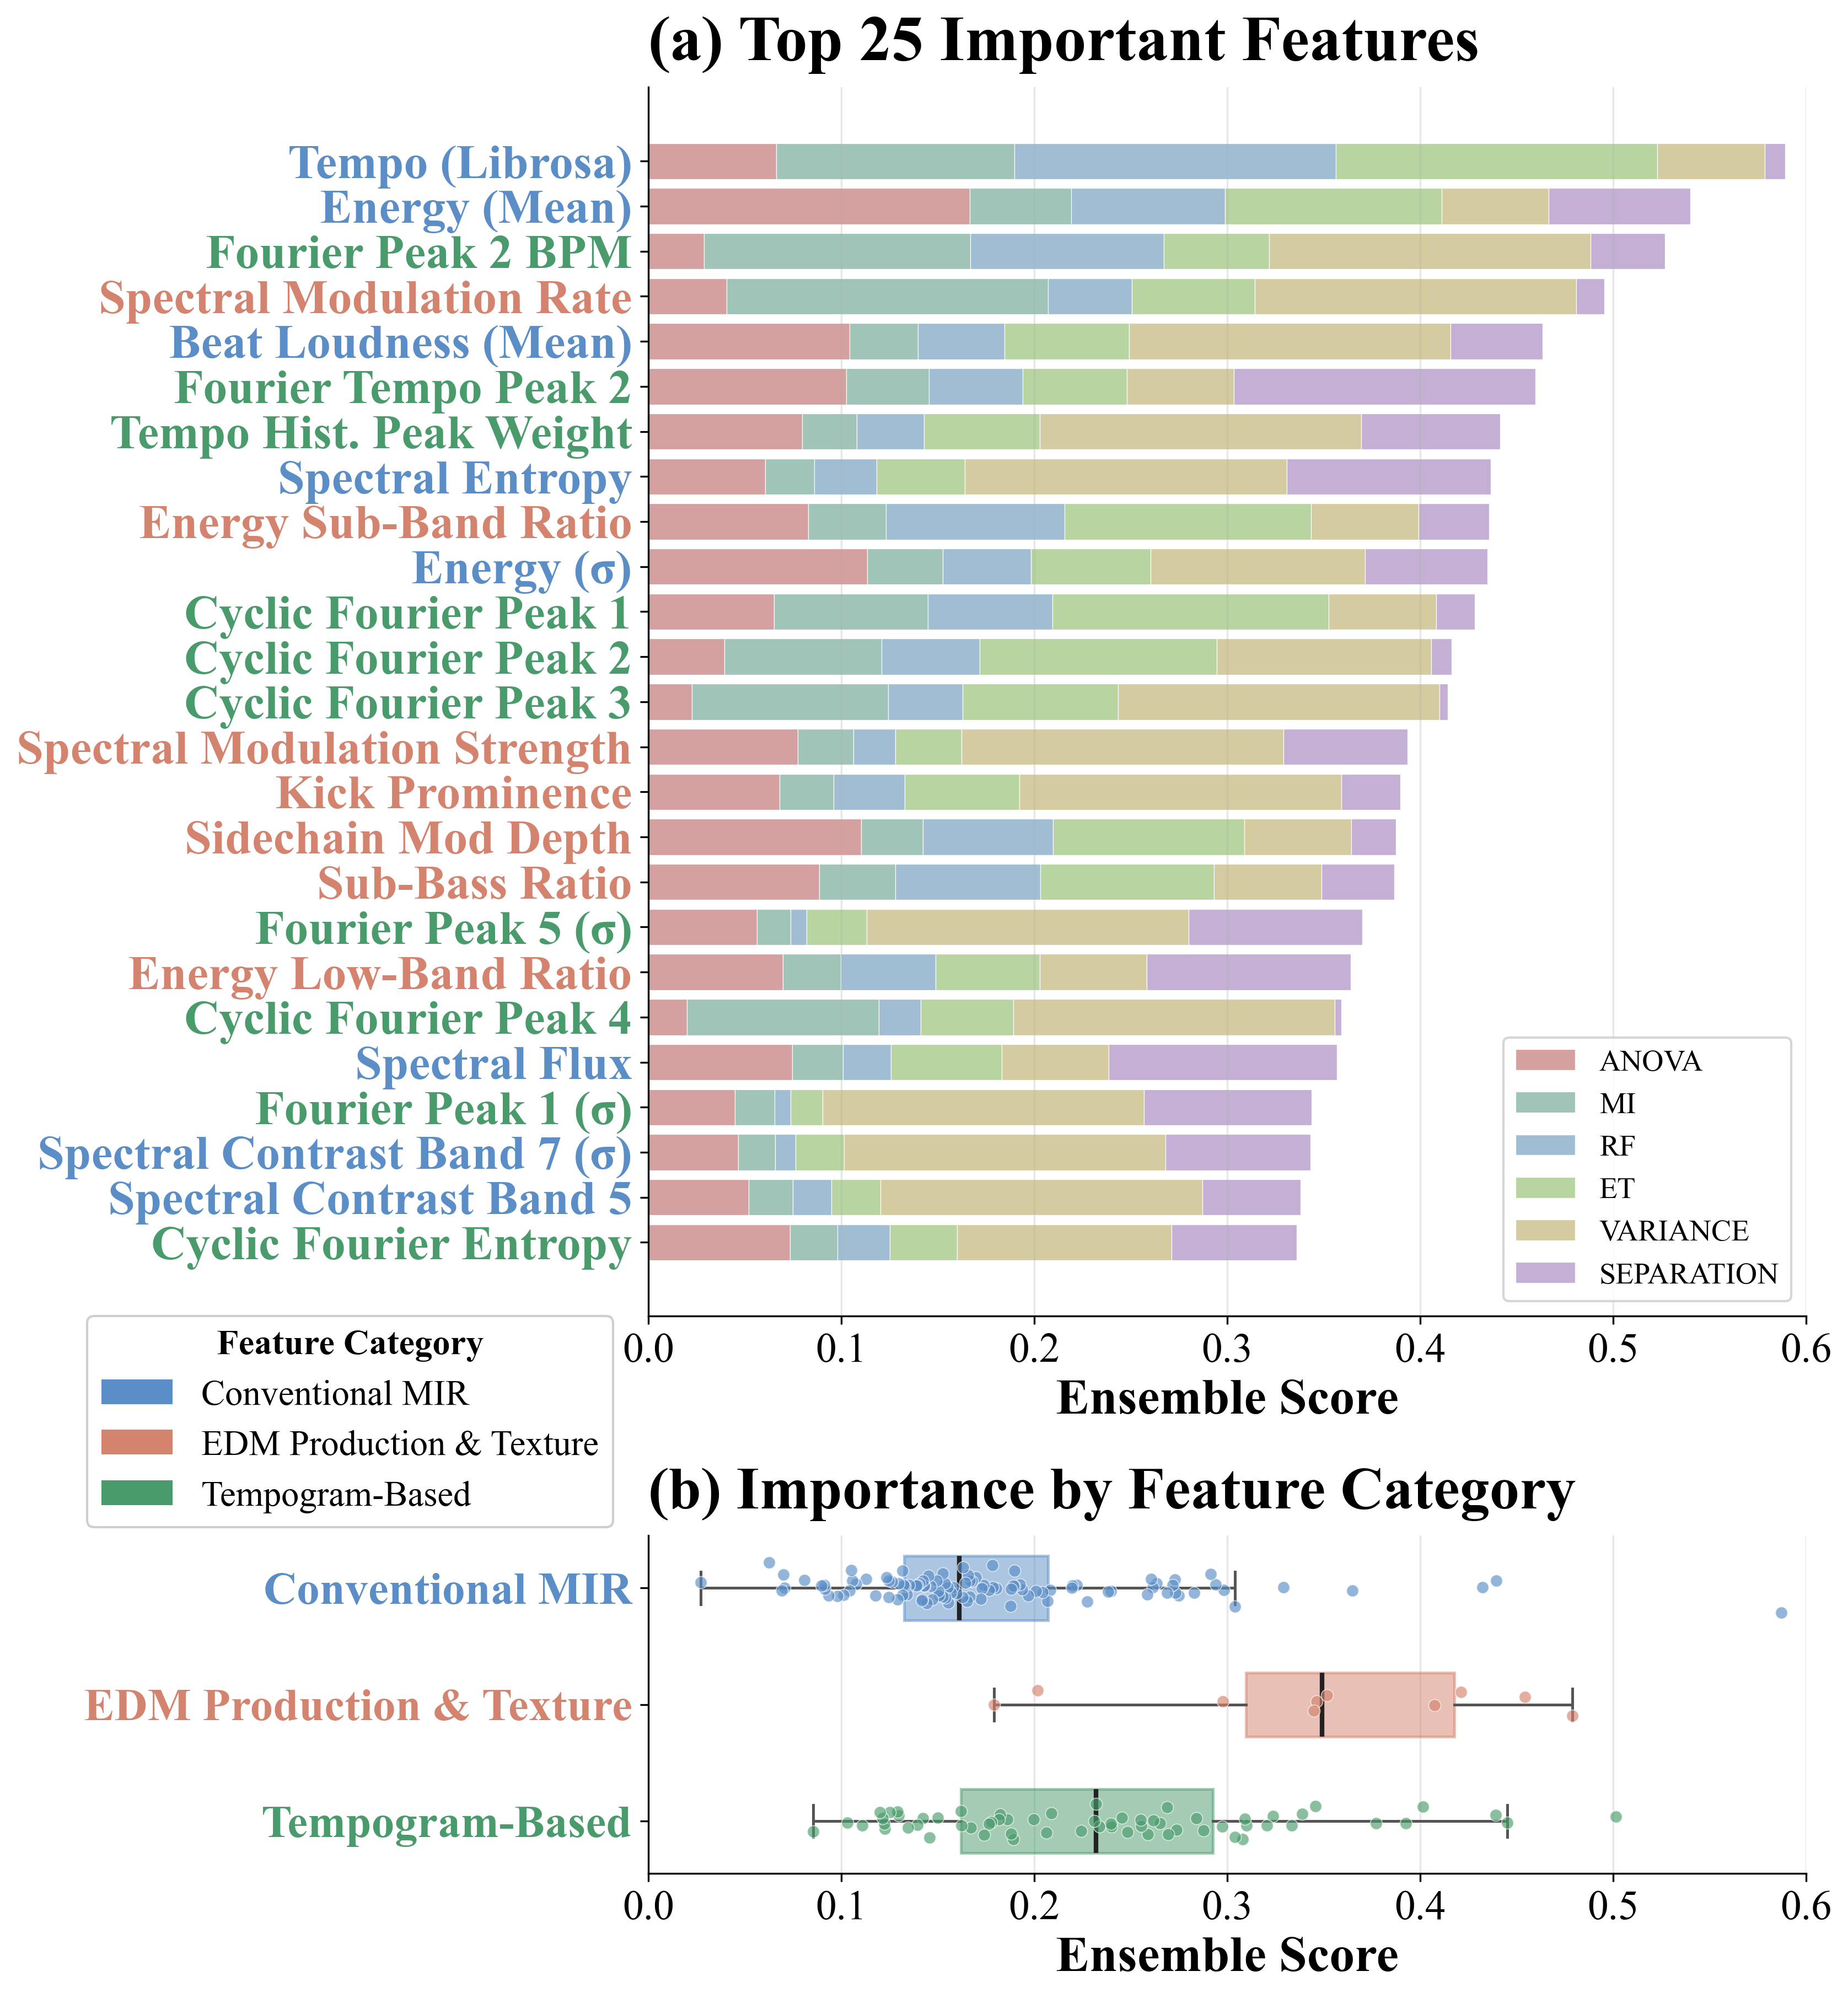
\includegraphics[width=\columnwidth]{figs/paper/fig2_feature_importance.png}
		\caption{Feature importance analysis. (a) Top-25 features ranked by an ensemble of evaluation metrics. (b) Importance distributions across feature categories. EDM-specific descriptors (Production \& Texture, Tempogram-based) substantially outperform standard MIR timbral features, confirming that genre identity in EDM is governed primarily by temporal evolution and mastering aesthetics rather than static spectral properties.}
		\label{fig:features}
	\end{figure}
    
	Figure~\ref{fig:features} reveals the discriminative power of our feature set, with rhythmic (BPM) and tempogram-derived descriptors dominating the top ranks. The greedy silhouette-optimized selection (Stage~1) exclusively selected tempogram and cyclic tempogram features, confirming that EDM's identity is defined less by static timbral or spectral properties and more by temporal evolution---build-ups, drops, and layered rhythmic patterns that shape its dancefloor functionality. The ensemble top-up (Stage~2) added energy and spectral modulation features, providing complementary genre-discriminative diversity.

	\subsection{Natural Clustering Structure}\label{ssec:natural}

	Since K-means yields the highest-quality clusters at $k$=35 and the consensus criteria for optimal-$k$ selection require sweeping over $k$ values---a procedure native to partitional methods---we adopt K-means for natural-$k$ discovery. When removing the $k$=35 constraint, equal-weight consensus of four validity criteria (silhouette, inertia elbow, Calinski-Harabasz, Davies-Bouldin; see Appendix~\ref{app:validation} for detailed curves) identifies $k$=20 as the optimal number of clusters. This optimal $k$=20 (and the surrounding 19--23 range across validation methods) confirms our core thesis mathematically: the commercial taxonomy is acoustically overspecified by over one-third.


	We emphasize that this finding concerns \emph{acoustic} overspecification and does not imply that the commercial taxonomy is inherently flawed. Genre labels serve cultural, historical, and commercial functions that extend well beyond acoustic separability---they encode community identity, regional scene affiliations, DJ set-programming conventions, and listener expectations shaped by years of cultural practice~\cite{brackett2016}. Two genres may be acoustically near-identical yet culturally distinct, and such distinctions are legitimate from a music-industry perspective---Appendix~\ref{app:convergent} illustrates several such ``acoustically convergent'' pairs whose radar profiles nearly overlap despite carrying different commercial labels. Our claim is narrower: when evaluated strictly on the basis of audio features, approximately one-third of the prescribed 35 categories lack sufficient acoustic differentiation to form distinct clusters, suggesting that the current taxonomy subdivides what are, acoustically, coherent styles.

	\subsubsection{Acoustic Topography: Purity, Concentration, and Size}

    \begin{figure*}[t]
		\centering
		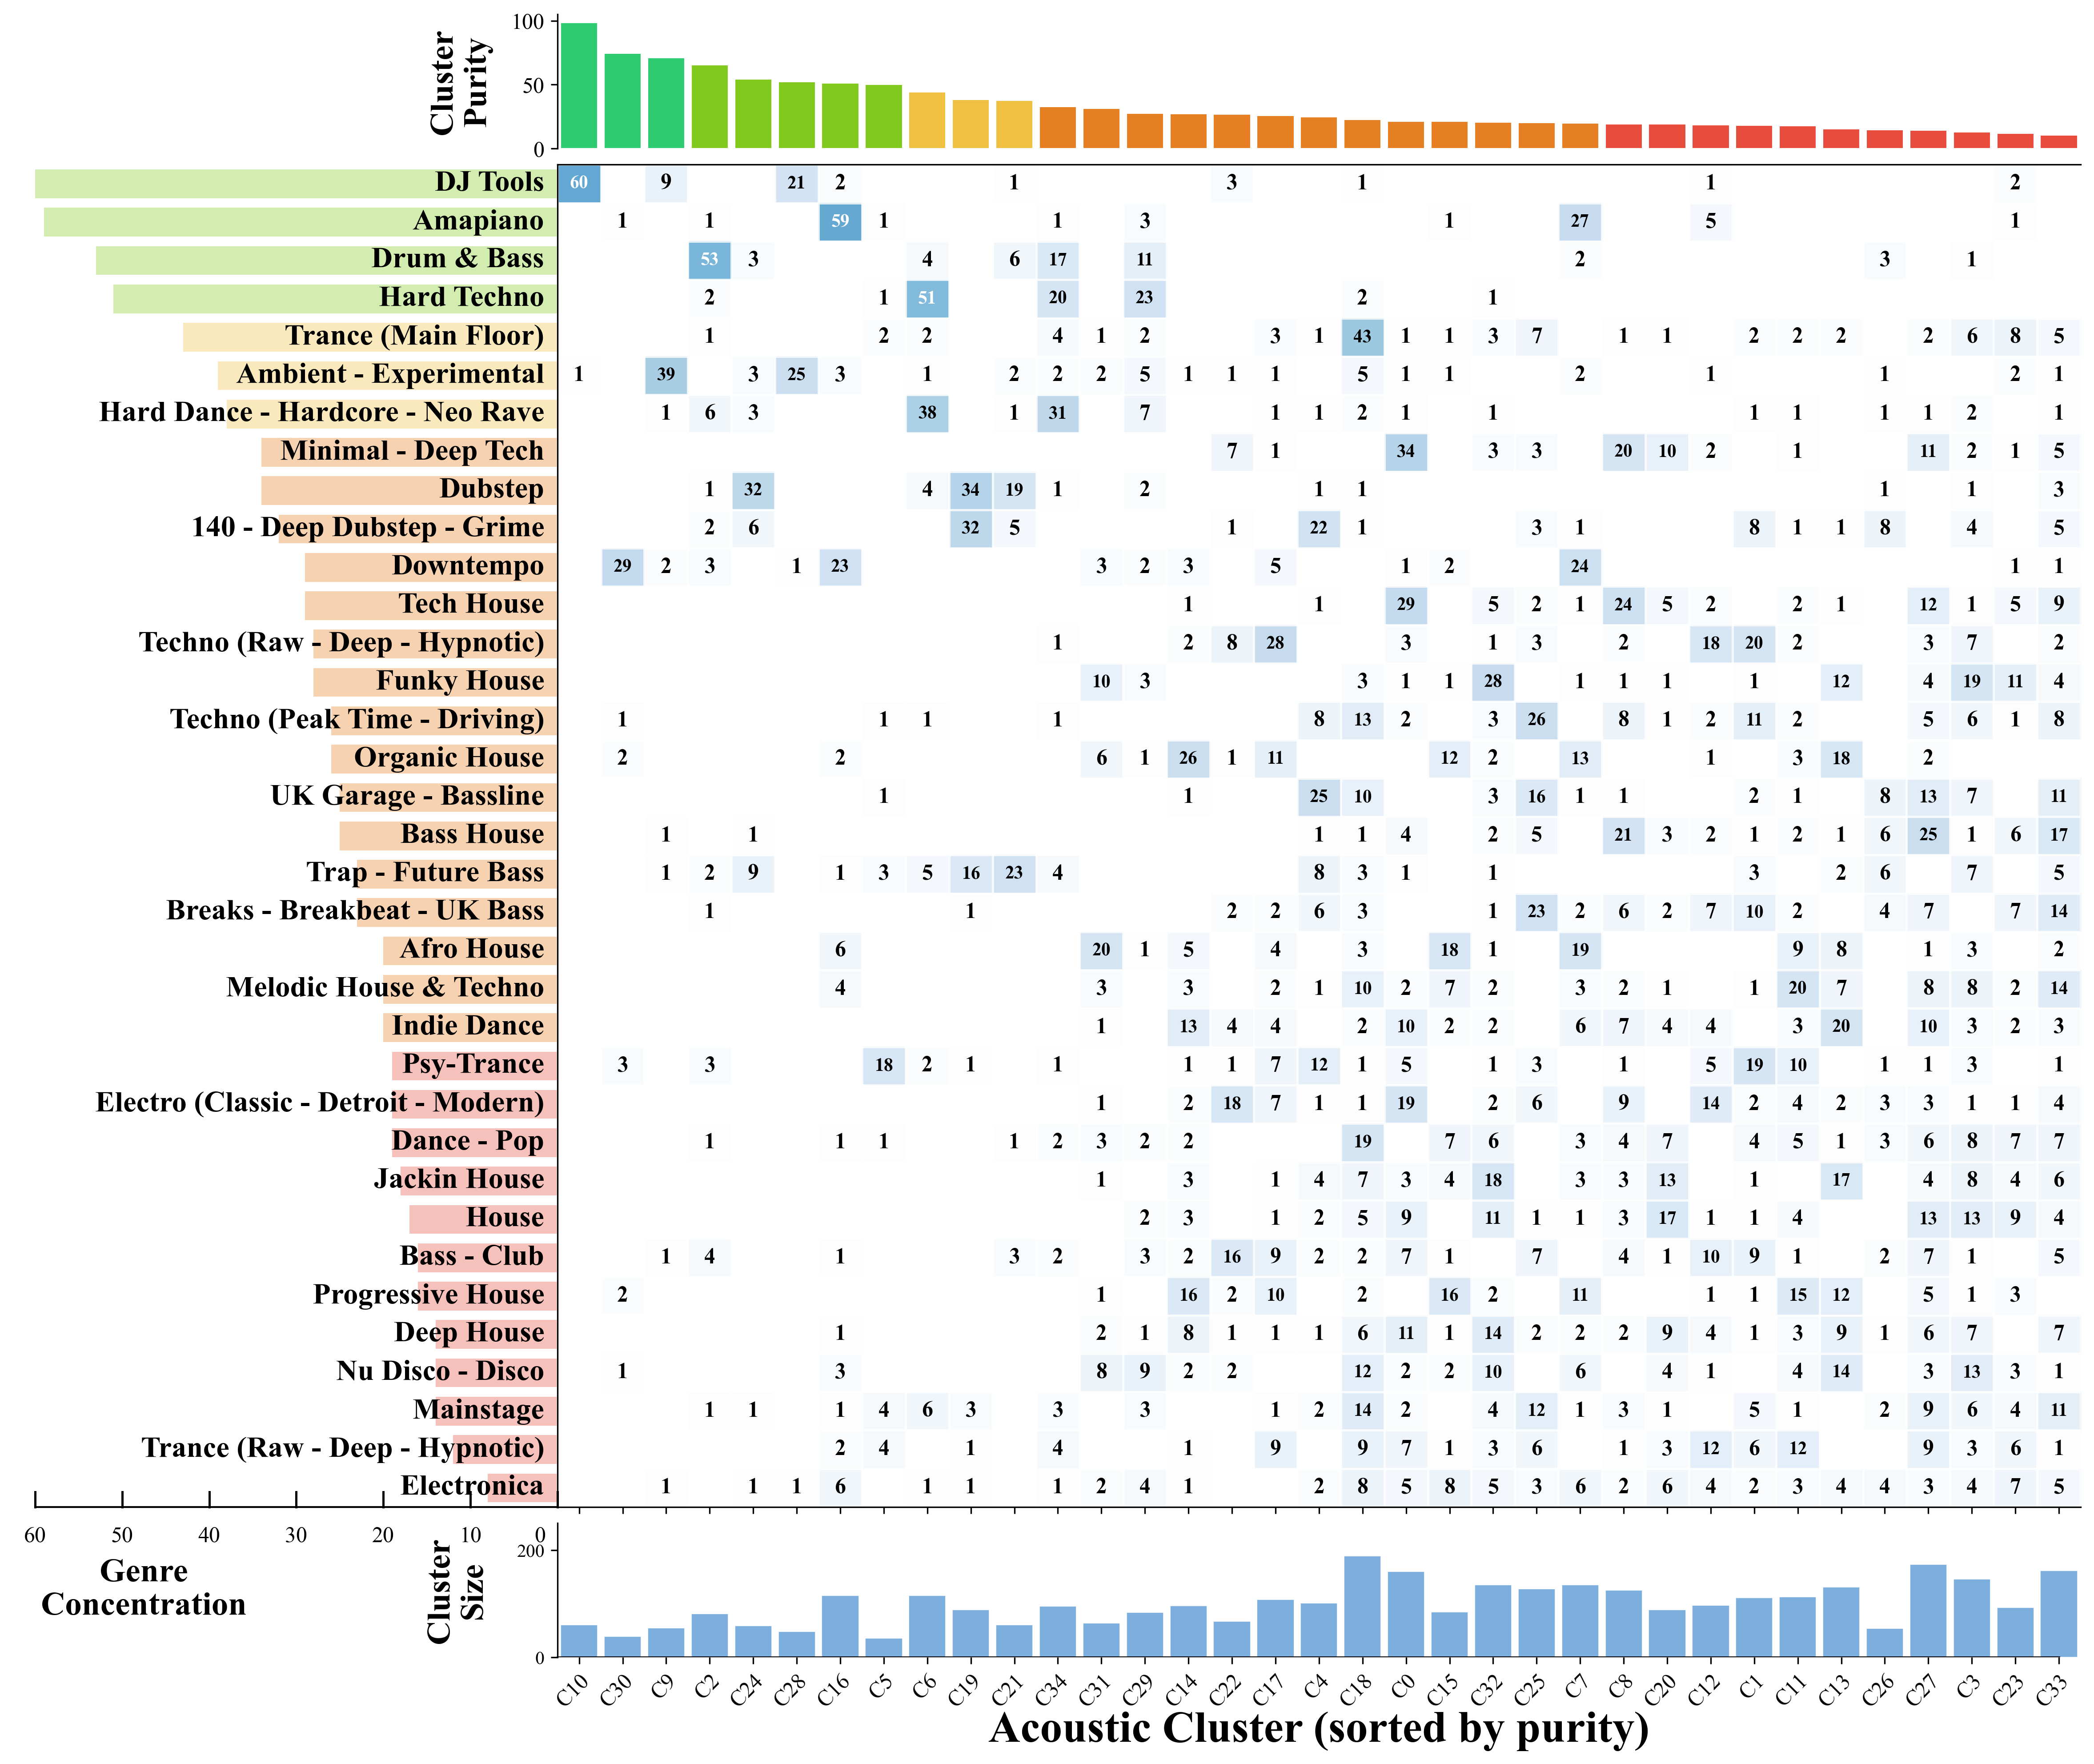
\includegraphics[width=\textwidth]{figs/paper/fig3_confusion_matrix.png}
		\caption{Confusion matrix mapping 35 commercial genre labels to 35 discovered acoustic clusters. The matrix is augmented by three marginals: \textit{Cluster Purity} (top) measures the acoustic exclusivity of a cluster; \textit{Genre Concentration} (left) measures how acoustically monolithic a commercial genre is; and \textit{Cluster Size} (bottom) indicates the total volume of tracks in that acoustic space. The clear inverse relationship between cluster size and purity highlights how massive, generic acoustic templates absorb multiple overlapping commercial labels, while smaller, pure clusters represent distinct sonic niches.}
		\label{fig:confusion}
	\end{figure*}

	Figure~\ref{fig:confusion} visualizes the mapping between commercial labels and acoustic clusters, augmented with three structural marginals: Cluster Purity, Cluster Size, and Genre Concentration. Analyzing these marginals reveals the complex typography of EDM, which transitions from distinct, isolated acoustic niches to generic stylistic melting pots.

	\textbf{Crystallized Niches (High Purity, High Concentration).} The upper-left quadrant of the ordered matrix reveals clusters with exceptional purity that are tightly mapped to highly concentrated genres like DJ Tools, Amapiano, and Drum \& Bass. In these cases, the commercial taxonomy perfectly mirrors acoustic reality. High genre concentration implies these styles are acoustically monolithic---producers adhere rigidly to a narrow set of defining sonic rules. Consequently, their resulting clusters are highly pure, forming isolated ``crystallized'' islands in the feature space that resist hybridization.

	\textbf{The Mainstream Melting Pot (Large Cluster Size, Low Purity).} Conversely, the largest clusters (shown in the bottom margin) consistently exhibit the lowest purity. These massive acoustic hubs act as ``liquid zones'' that absorb tracks from heavily overlapping commercial categories---such as Tech House, Minimal--Deep Tech, and generic House. The inverse relationship between cluster size and purity implies the existence of a shared mainstream acoustic template. The industry artificially fragments this unified sonic space into multiple micro-genres for marketing and curation purposes, even though the tracks are acoustically indistinguishable at a structural level.

	\textbf{Acoustic Fragmentation (Low Genre Concentration).} The left margin reveals genres with exceedingly low concentration, meaning their tracks are dispersed across numerous distinct acoustic clusters. Broad labels or heavily evolving genres often fail to localize into a single acoustic signature. This fragmentation implies that the commercial label functions as a cultural umbrella term for contradictory production styles that our clustering correctly partitions. Ultimately, the interplay of these three metrics demonstrates that EDM taxonomy is not uniformly overspecified; rather, overspecification is heavily concentrated in the mainstream center, while the stylistic periphery remains acoustically crisp.

	\subsubsection{Genre Purity and Acoustic Extremity}

	To summarize each cluster's acoustic signature, we assign every extracted feature to one of six interpretable dimensions---Energy, Danceability, Tempo, Harmonic complexity, Rhythmic density, and Electronic texture---via an explicit, manually curated mapping that covers all features in the dataset (Section~\ref{ssec:features}), including the EDM-specific production descriptors. Within each dimension, features are z-score normalized before averaging so that all contribute equally regardless of scale. Each cluster's per-dimension mean is then scaled to 0--100 via \mbox{$p_5$/$p_{95}$} linear interpolation across the full corpus and clipped to $[0,100]$.

	Figure~\ref{fig:profiles} reveals that genre purity correlates with acoustic extremity. The purest clusters occupy feature-space vertices: DJ Tools---a utility category of loops, samples, and mixing elements---maximizes Electronic texture while minimizing other dimensions, and its tracks span multiple clusters precisely because the category encompasses diverse production styles. Similarly, Ambient-dominated clusters push Harmonic features to extremes while compressing Rhythmic and Energy dimensions. These poles---whether functional (DJ Tools) or artistic (Ambient)---demonstrate how specialized production constraints create acoustic signatures that resist genre hybridization.

	Conversely, the most mixed clusters exhibit moderate, overlapping profiles rather than converging to a single ``neutral'' center. Each hybrid style draws on parent traditions differently---bass-heavy clusters extend along Rhythmic and Electronic axes, while groove-oriented clusters balance Danceability and Energy---suggesting that genre blending follows multiple distinct pathways through the feature space.

	\begin{figure}[t]
		\centering
		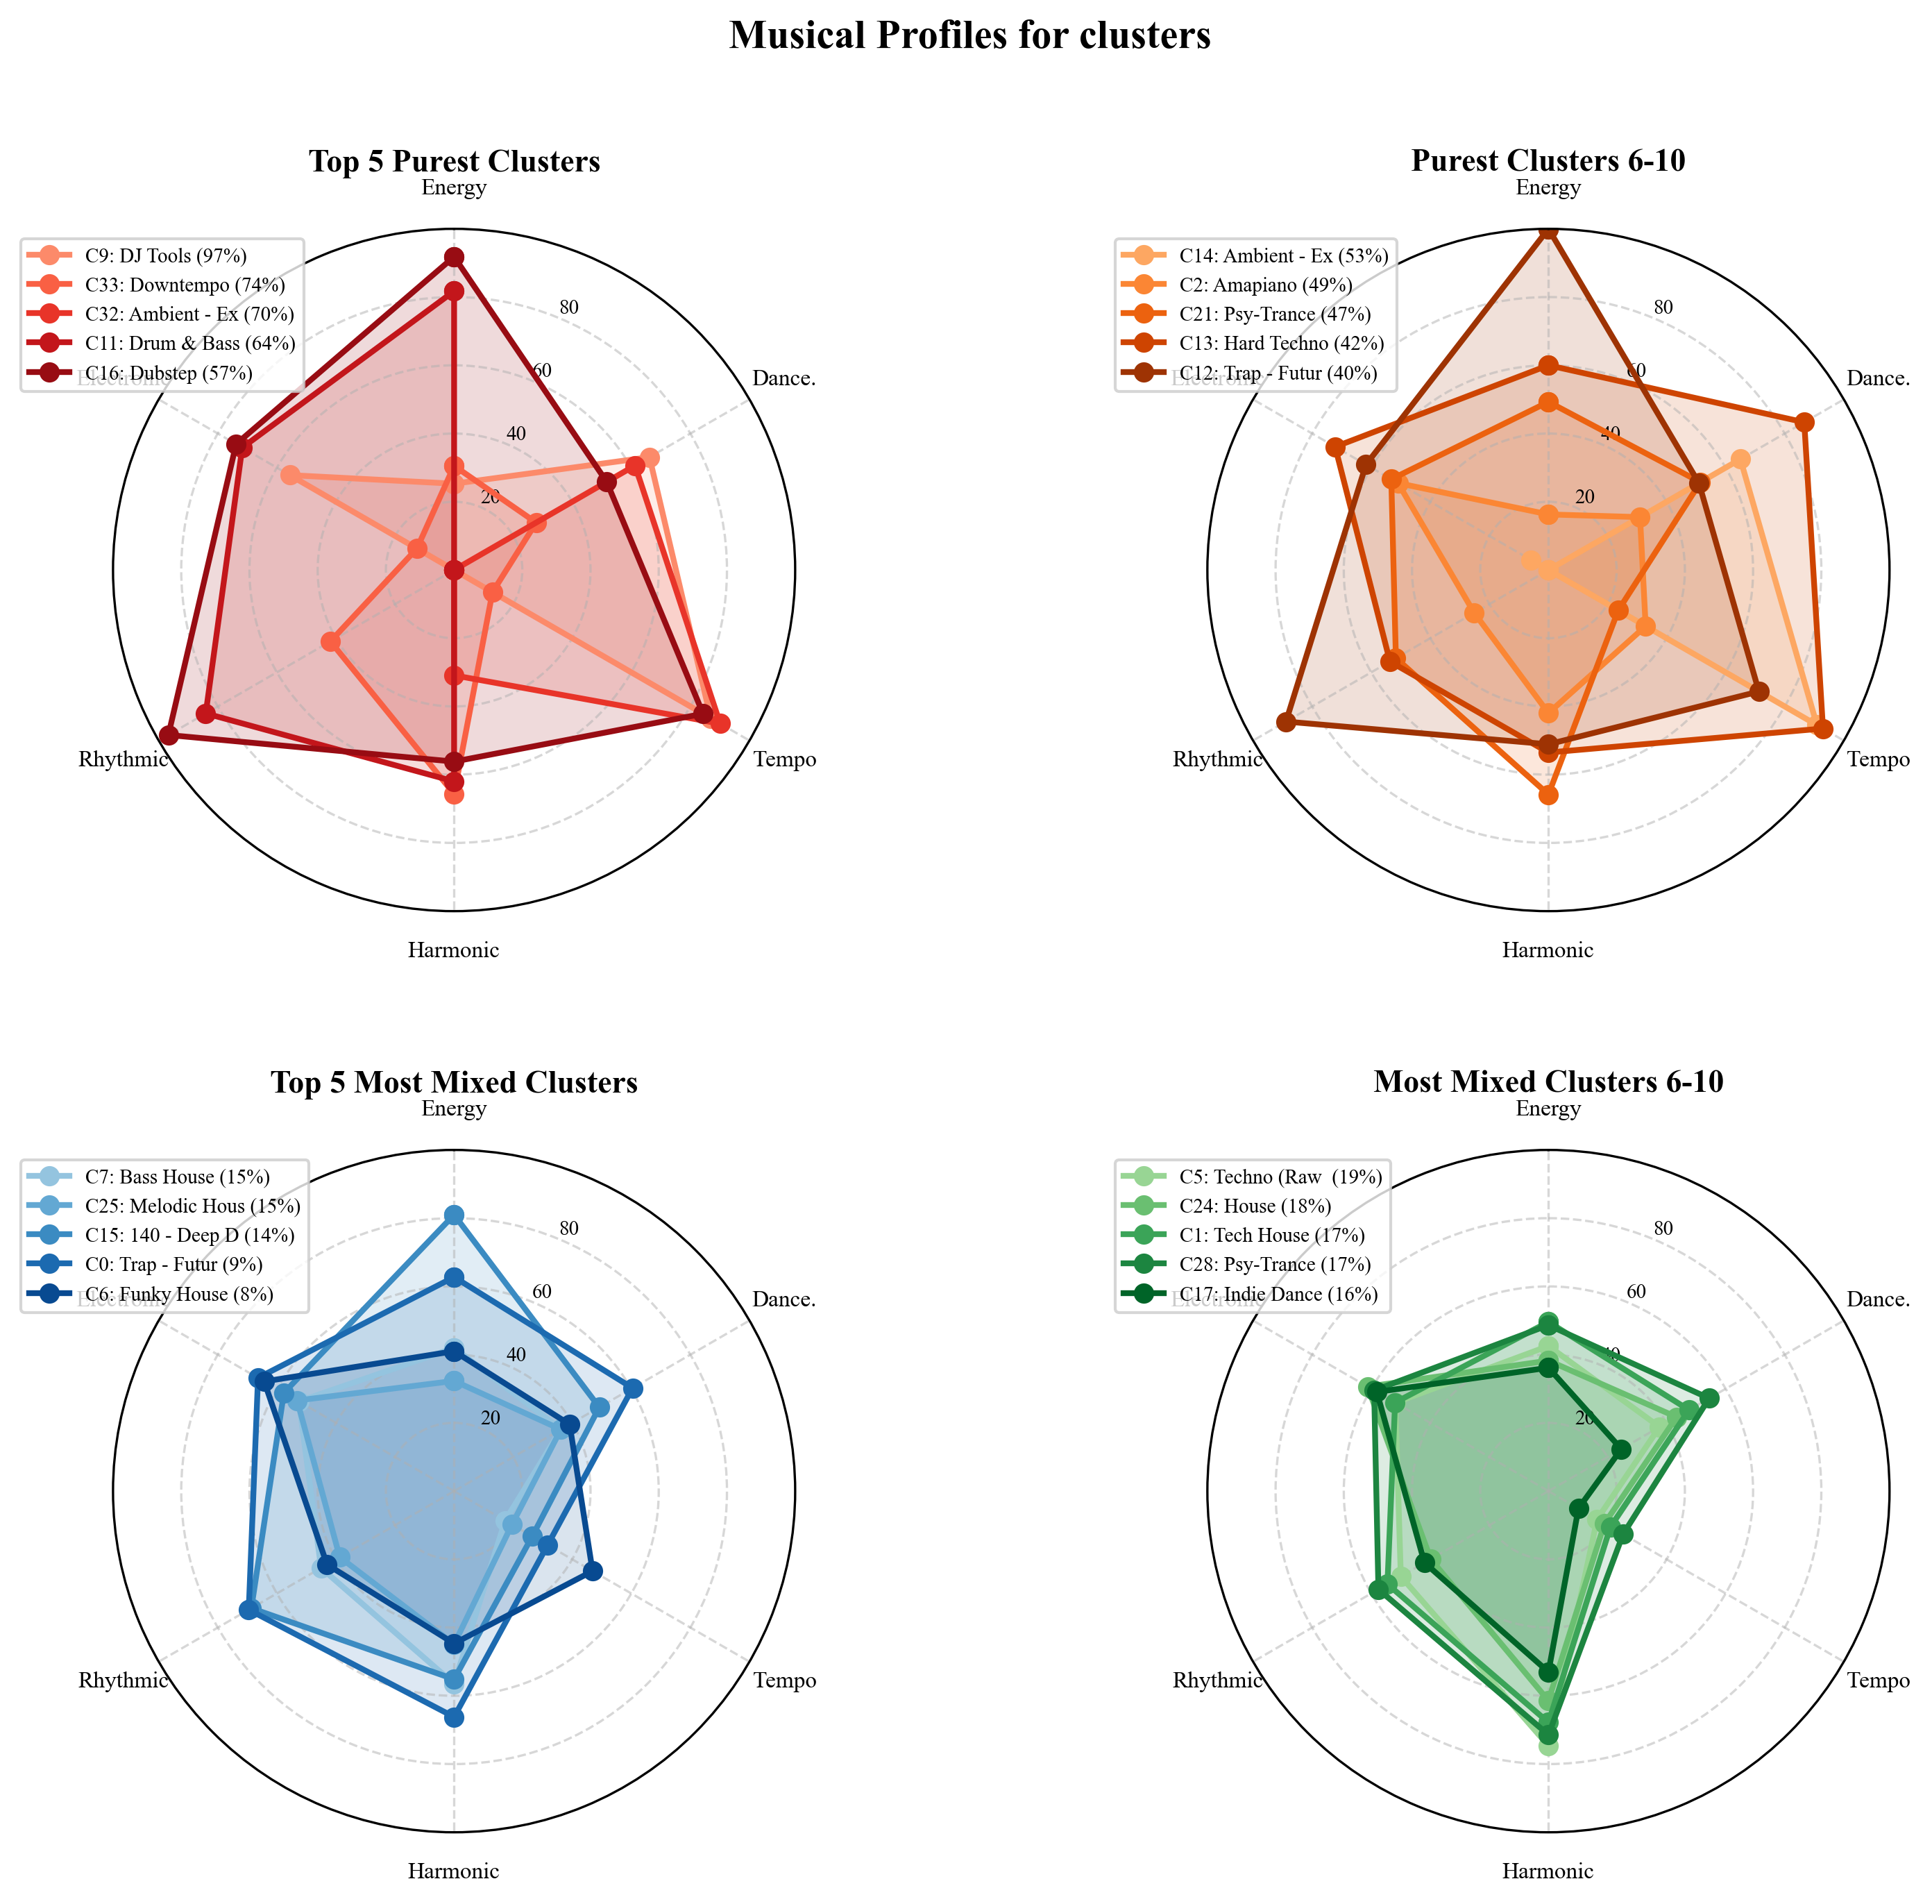
\includegraphics[width=0.95\columnwidth]{figs/paper/fig4_musical_profile.png}
		\caption{Acoustic archetypes of the purest versus most hybridized clusters. Each vertex aggregates z-score-normalized features into one of six dimensions: Energy (RMS, loudness, dynamic range, energy ratios), Danceability (danceability, beat regularity, sidechain modulation), Tempo (BPM, tempo histogram peaks), Harmonic (chroma vectors, harmonic-to-percussive ratio), Rhythmic (onsets, percussive density, kick prominence, tempogram strengths), and Electronic texture (spectral shape, MFCCs, spectral contrast, sub-bass ratio). Values are scaled to 0--100 via $p_5$/$p_{95}$ interpolation. Pure clusters (e.g., DJ Tools, Ambient) localize at feature extremes, highlighting highly specialized production constraints, whereas hybrid mainstream clusters exhibit moderate, overlapping acoustic profiles.}
		\label{fig:profiles}
	\end{figure}


	\subsubsection{Implications for Genre Organization}

	The pattern observed in Figure~\ref{fig:profiles} suggests EDM operates through two distinct modes: ``crystallized'' genres at acoustic extremes maintaining distinct identities through specialized production choices, and ``liquid'' zones in the center enabling creative exploration and genre evolution. The improvement in clustering quality when allowing natural groupings ($k$=20 vs $k$=35) combined with these purity patterns indicates that many commercial genre distinctions may subdivide what are acoustically coherent styles, while genuine acoustic boundaries occur at the extremes where production techniques diverge most dramatically.

	This finding suggests that effective music information retrieval should account for this core-periphery structure, where genre boundaries are clearest at the extremes but deliberately blurred in the hybrid center.


	\subsection{Hierarchical Genre Structure}\label{ssec:hierarchy}

	\begin{figure}[!t]
		\centering
		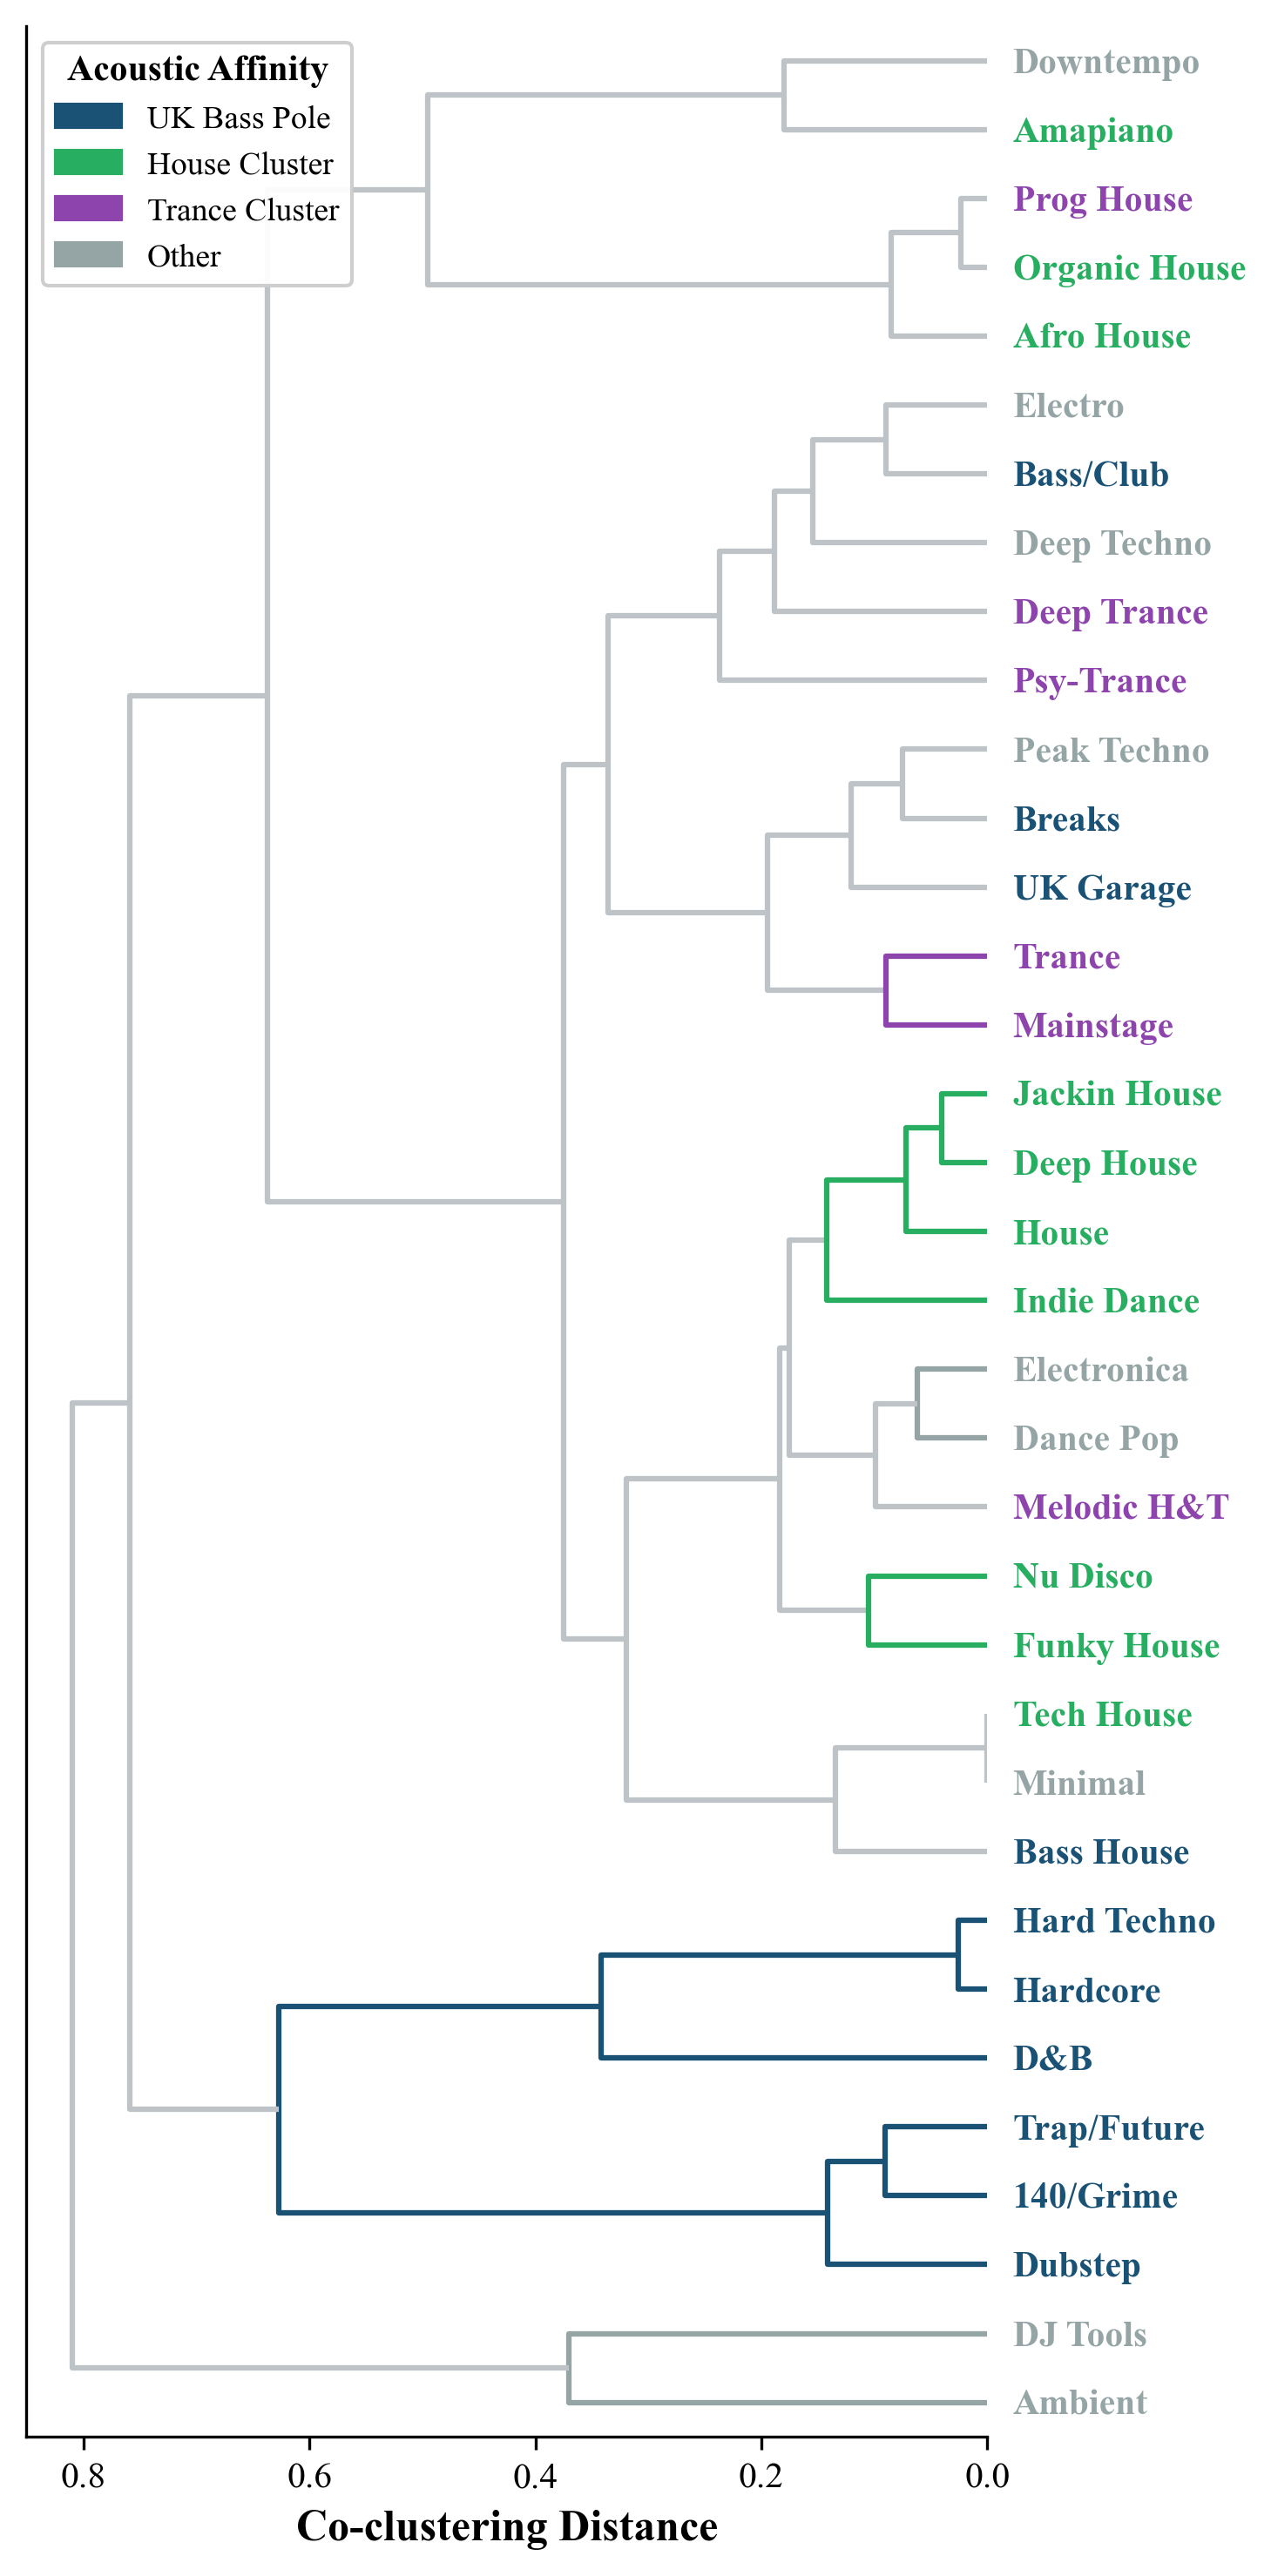
\includegraphics[width=0.45\textwidth]{figs/paper/fig5_dendrograms.png}
		\caption{Hierarchical genre lineage derived from co-clustering affinity ($1-\hat{a}_{ij}$, where $\hat{a}_{ij}$ is the normalized co-clustering frequency across 50 K-means restarts). The dendrogram exposes two rigid acoustic poles---a tightly knit UK Bass cluster and isolated functional/atmospheric outliers---separated by a massive middle gradient where house, trance, and techno variants indiscriminately interleave, proving the continuous nature of the mainstream acoustic space.}
		\label{fig:dendrograms}
	\end{figure}
    
	To reveal hierarchical structure, we compute a \emph{co-clustering affinity} between every genre pair: across 50 independent K-means runs ($k$=35), we count how often tracks from two genres land in the same cluster, normalized by genre size. Converting affinity to distance ($1-\hat{a}_{ij}$) and applying average linkage yields the dendrogram in Figure~\ref{fig:dendrograms}. The resulting tree reveals that EDM's acoustic space is organized not as a set of discrete genre families but as a gradient between two poles, separated by a broad middle zone where most commercial labels overlap.

	\textbf{The UK Bass Pole.} At one extreme of the dendrogram, Drum \& Bass, Dubstep, 140/Grime, Hard Techno, and Hardcore form a tightly interconnected cluster that merges internally before joining any other genres. This cohesion is consistent with Reynolds' ``hardcore continuum'' thesis~\cite{reynolds2013energy}: shared production techniques---chopped breaks, sub-bass emphasis, and syncopated rhythms at related tempos (70/140/170\,BPM as octave equivalents)---create a distinct acoustic signature that resists hybridization.

	\textbf{The Functional/Atmospheric Pole.} At the opposite extreme, DJ Tools and Ambient occupy isolated positions, merging last with the rest of the taxonomy. These categories are defined by specialized production constraints (utility loops and atmospheric textures, respectively) that place them at feature-space vertices, far from the mainstream.

	\textbf{The Middle Gradient.} Between these poles lies a large, densely connected zone where house, trance, and techno variants interleave rather than forming self-contained blocks. Core house sub-clusters emerge (Deep House--House--Jackin House; Nu Disco--Funky House), as does a Trance--Mainstage pair, but these merge with non-sibling genres (e.g., Deep Trance clusters with Deep Techno; Breaks and UK Garage sit near Peak Techno; Melodic House \& Techno neighbours Indie Dance) before consolidating with their supposed families. This interleaving is the strongest structural evidence of overspecification: the commercial taxonomy imposes discrete boundaries on what the acoustic signal reveals to be a continuous gradient. The labels that fragment this middle zone---Tech House vs.\ Minimal, Progressive House vs.\ Melodic House \& Techno---subdivide acoustically overlapping styles for cultural and curatorial rather than acoustic reasons.





	\section{Conclusion}\label{sec:conclusion}
	We presented an unsupervised approach to analyzing EDM taxonomy through clustering with audio descriptors. A key challenge was the absence of established guidelines for EDM feature design; we addressed this by constructing a tailored acoustic feature space spanning spectral-harmonic, production, texture, and rhythmic dimensions. Our findings indicate that natural acoustic clustering produces over one-third fewer distinct groups than commercial taxonomy suggests (20 compared to 35), with convergent evidence from pre-trained embeddings validating this overspecification.

	This work contributes to understanding the relationship between acoustic properties and genre labels. Genre categories naturally emerge from artist and community practice before being codified into fixed taxonomies by distributors like Beatport. Our results suggest that this codification process preserves more distinctions than the acoustic signal warrants---raising the broader hypothesis that genre labels, whether community-driven or commercially curated, tend toward overspecification when cultural and acoustic criteria are conflated. MIR systems might therefore benefit from hierarchical approaches that explicitly decouple acoustic similarity from commercial categorization. For instance, a two-tier architecture mapping broad acoustic clusters to specific commercial labels could optimize both computational efficiency and user navigation.

	Our analysis has two key limitations. First, it focuses solely on acoustic features and does not capture the cultural, historical, or scene-level factors that legitimately motivate genre distinctions. Second, many EDM genres differ through subtle timbral and production-level cues---drum-machine palettes, synthesizer families, bass modulation patterns, and genre-specific groove micro-timing---that may not be fully resolved by our feature set. Genre merging in our clustering may therefore partly reflect insufficient feature granularity rather than genuine acoustic equivalence. Future work should investigate whether fine-grained timbral descriptors (e.g., modulation spectral features, synthesis-aware representations) can recover distinctions that our current features miss, and whether incorporating cultural metadata yields a richer picture of genre organization.

	\begin{acknowledgments}
		The authors would like to thank Jingbang Liu for developing the web scraping infrastructure used for systematic data collection from Beatport, and Haotian Fang for productive discussions regarding feature selection. Their contributions were instrumental to this research.
	\end{acknowledgments}

	%%%%%%%%%%%%%%%%%%%%%%%%%%%%%%%%%%%%%%%%%%%%%%%%%%%%%%%%%%%%%%%%%%%%%%%%%%%%%
	%bibliography here
	\bibliography{smc2026bib}

	\clearpage
	\appendix
	\section{Feature Taxonomy}\label{app:features}

	Table~\ref{tab:feature_taxonomy} maps each feature category to its musicological significance and EDM production relevance, providing context for why these features were selected.

	\begin{table*}[t]
		\centering\small
		\caption{Taxonomy of the 194 acoustic features. This mapping bridges low-level signal processing (Feature) with theoretical concepts (Musicological Significance) and practical mixing conventions (EDM Production Relevance), demonstrating how cultural genre rules manifest acoustically.}
		\label{tab:feature_taxonomy}
		\begin{tabular}{p{1.9cm}p{4.3cm}p{4.2cm}p{4.4cm}}
			\toprule
			\textbf{Category} & \textbf{Feature} & \textbf{Musicological Significance} & \textbf{EDM Production Relevance} \\
			\midrule
			\multicolumn{4}{l}{\textbf{Conventional MIR}} \\
			\midrule
			Timbral & Spectral centroid, spread, entropy, flux, rolloff; MFCCs; ZCR; energy \& energy entropy; spectral flatness \& bandwidth
			& Captures Smalley's spectral space---brightness, density, and the dynamic evolution of synthesized sounds.
			& Distinguishes filter automation in Deep House from distortion profiles in Dubstep; identifies synthesis methods (analog vs.\ FM). \\
			\addlinespace
			Rhythmic & Tempo/BPM \& histograms; autocorrelation-derived danceability; frequency-band beat emphasis; onset rate
			& Tempo as a primary cultural signifier---from House's 120--130\,BPM to D\&B's 160--180\,BPM; quantifies groove mechanics.
			& Broad genre boundaries dictated by BPM limits; beat-band profiles reveal sub-bass drops (Trap / Bass) vs.\ mid-range punch (Techno). \\
			\addlinespace
			Harmonic & Chroma vectors; chroma deviation
			& Maps tonal vocabularies and harmonic stasis---essential for EDM's modal and repetitive practices.
			& Distinguishes modal, drone-based Techno from jazz-influenced Liquid D\&B; measures repetition vs.\ functional harmonic progression. \\
			\midrule
			\multicolumn{4}{l}{\textbf{Production and Texture}} \\
			\midrule
			Dynamics \& Texture & H/P ratio, crest factor, sub-bass ratio, sidechain proxy, spectral contrast, RMS statistics, dynamic range, energy variance, spectral modulation, kick prominence
			& Quantifies the mastering footprint, timbral sharpness, and large-scale structural energy (e.g., 8-bar variance).
			& Captures brickwall compression (the loudness war), sub-woofer focus, sidechain ducking aesthetics, and structural drops. \\
			\midrule
			\multicolumn{4}{l}{\textbf{Tempogram-based}} \\
			\midrule
			Temporal & Fourier, autocorrelation, and cyclic tempograms
			& Rhythmic spectrogram capturing localized tempo evolution and interlocking periodicities over time.
			& Reveals build-up acceleration and breakdown deceleration; identifies half-time/double-time rhythmic switches (Dubstep vs.\ D\&B). \\
			\bottomrule
		\end{tabular}
	\end{table*}



	\section{Cluster Validation Curves}\label{app:validation}

	Figure~\ref{fig:validation} shows how each of the four validity criteria evolves across $k$=10--30: silhouette score plateaus around $k$=18--20 while inertia and Davies-Bouldin reach elbow points near $k$=20, confirming that further splitting yields diminishing returns.

	\begin{figure}[t]
		\centering
		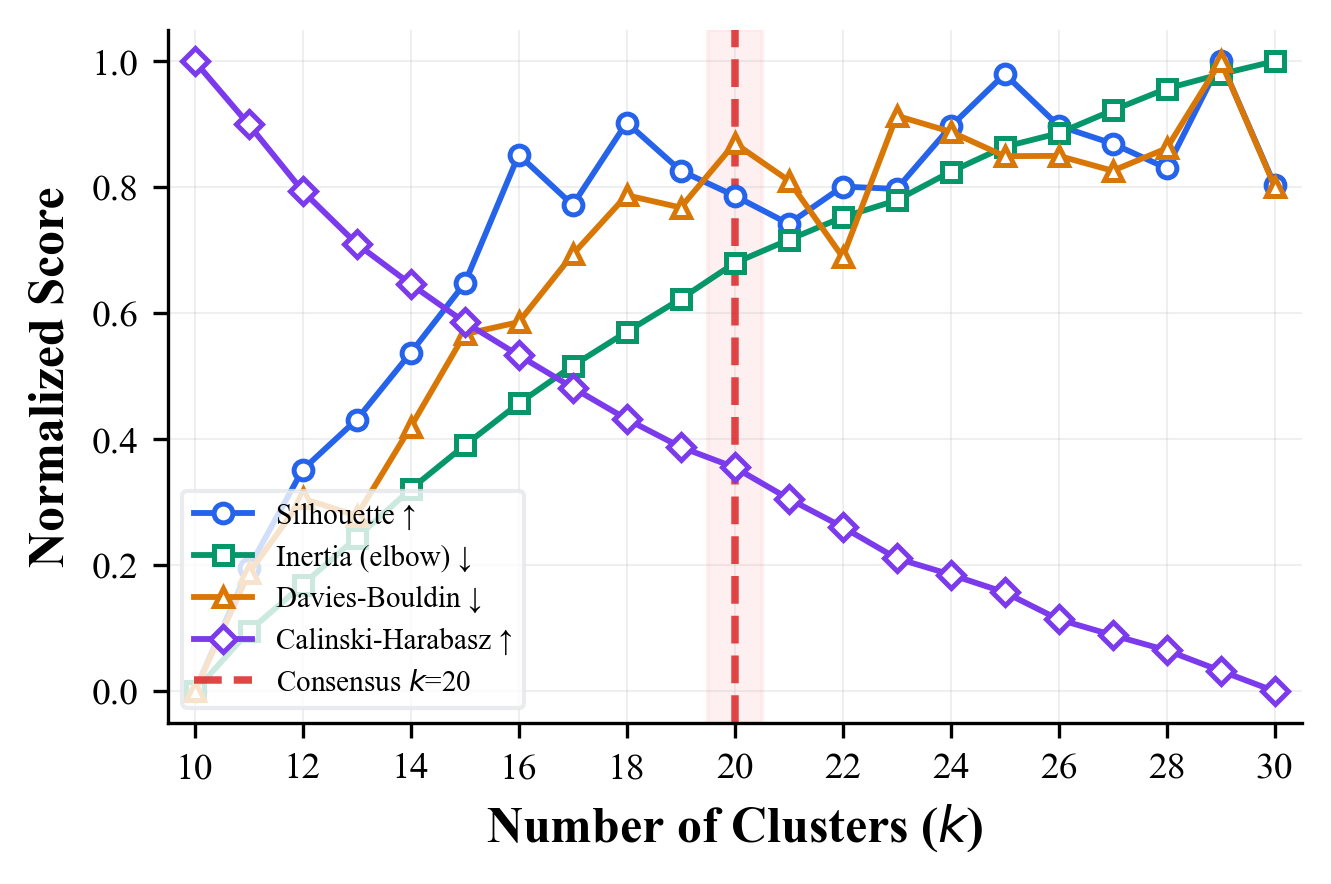
\includegraphics[width=0.95\columnwidth]{figs/paper/figa2_natural_k_validation.png}
		\caption{Natural cluster discovery across $k \in [10, 30]$. The vertical dashed line marks the consensus global optimum at $k$=20, determined by equal-weight voting of the critical inflection (elbow) points across all four structural validity criteria.}
		\label{fig:validation}
	\end{figure}

	\section{DJ Tools Sensitivity Analysis}\label{app:sensitivity}

	To verify that including DJ Tools---a utility category rather than a traditional genre---does not distort our findings, we re-ran the natural-$k$ consensus procedure after excluding all 100 DJ Tools tracks. The four validity criteria individually voted for $k \in \{16, 18, 21, 22\}$ (a four-way tie, resolved to $k$=16 by the tie-breaking rule), compared with the original votes of $k \in \{20, 20, 23, 25\}$ (clear consensus at $k$=20). Figure~\ref{fig:sensitivity} shows that the metric curves with and without DJ Tools are nearly overlapping, confirming that this utility category has negligible influence on the cluster-quality landscape. The individual criterion votes without DJ Tools bracket the original $k$=20 result (range 16--22, median 19.5), and the apparent shift to $k$=16 reflects tie-breaking mechanics rather than a genuine structural difference in the data.

	\begin{figure}[!t]
		\centering
		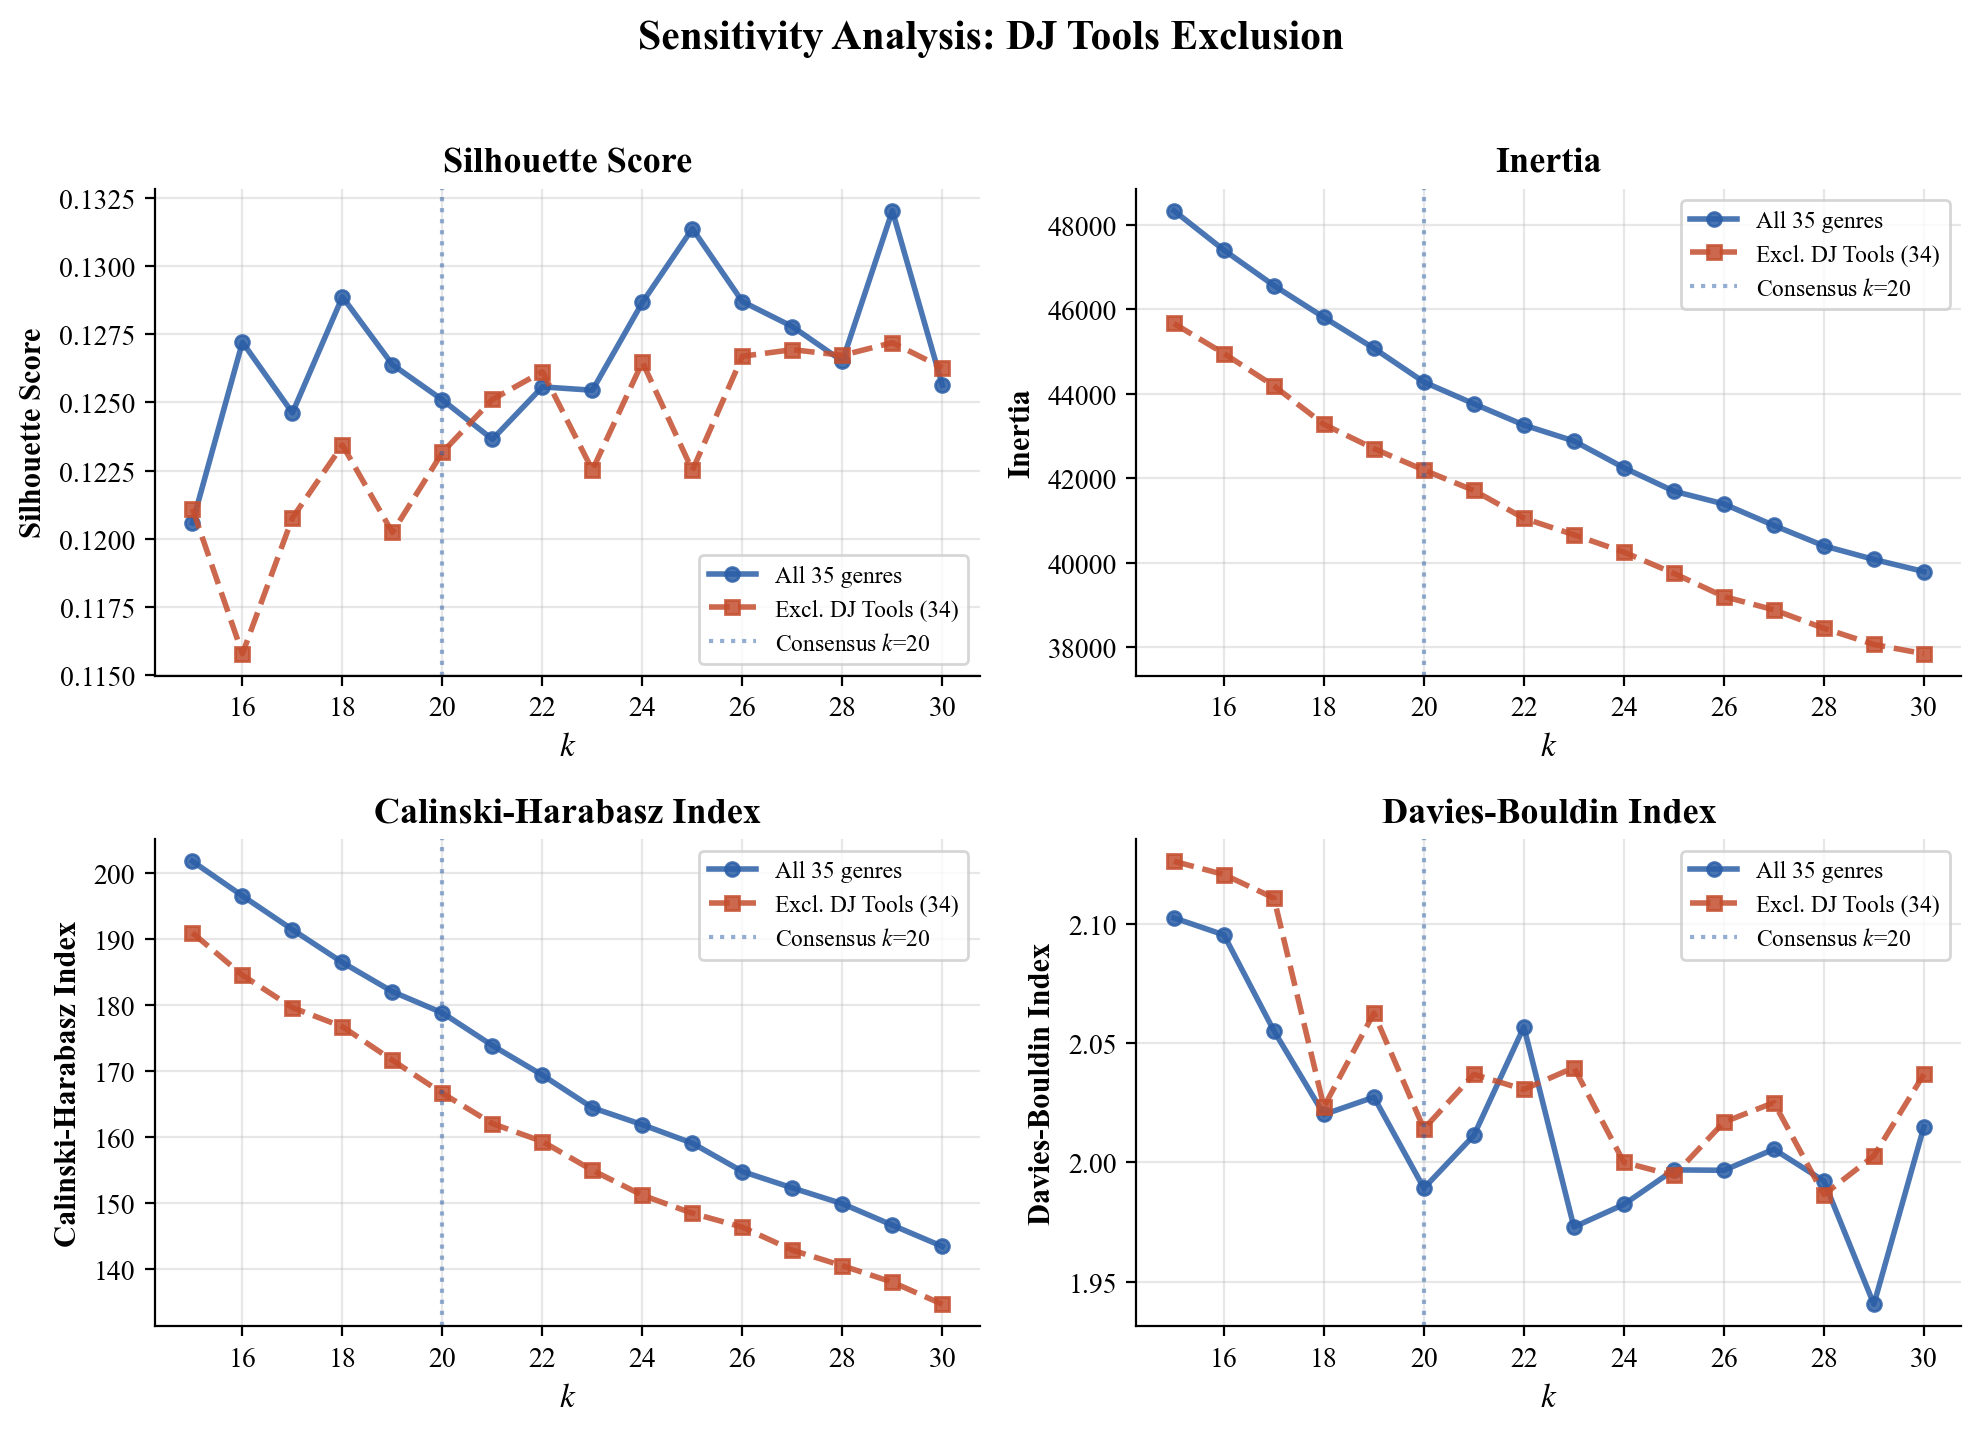
\includegraphics[width=0.95\columnwidth]{figs/paper/figa3_sensitivity_dj_tools.png}
		\caption{Sensitivity analysis isolating the structural impact of the ``DJ Tools'' utility category. Global metric curves fundamentally overlap whether DJ Tools are included (blue) or excluded (orange), confirming that this functional category does not distort the underlying optimal-$k$ consensus.}
		\label{fig:sensitivity}
	\end{figure}

	\section{Acoustically Convergent Genre Pairs}\label{app:convergent}

	To identify genre pairs that are acoustically near-indistinguishable despite carrying distinct commercial labels, we apply a dual filter: (1) high co-clustering rate under K-means ($k$=35, 50 restarts), requiring that tracks from the two genres frequently land in the same cluster; and (2) a profile difference $\Delta < 15$, computed as the mean absolute difference across the six radar dimensions in Figure~\ref{fig:profiles}. Of 595 possible genre pairs, 273 pass the $\Delta$ threshold; applying the co-clustering filter yields the top convergent pairs shown in Figure~\ref{fig:convergent}.

	\begin{figure}[!t]
		\centering
		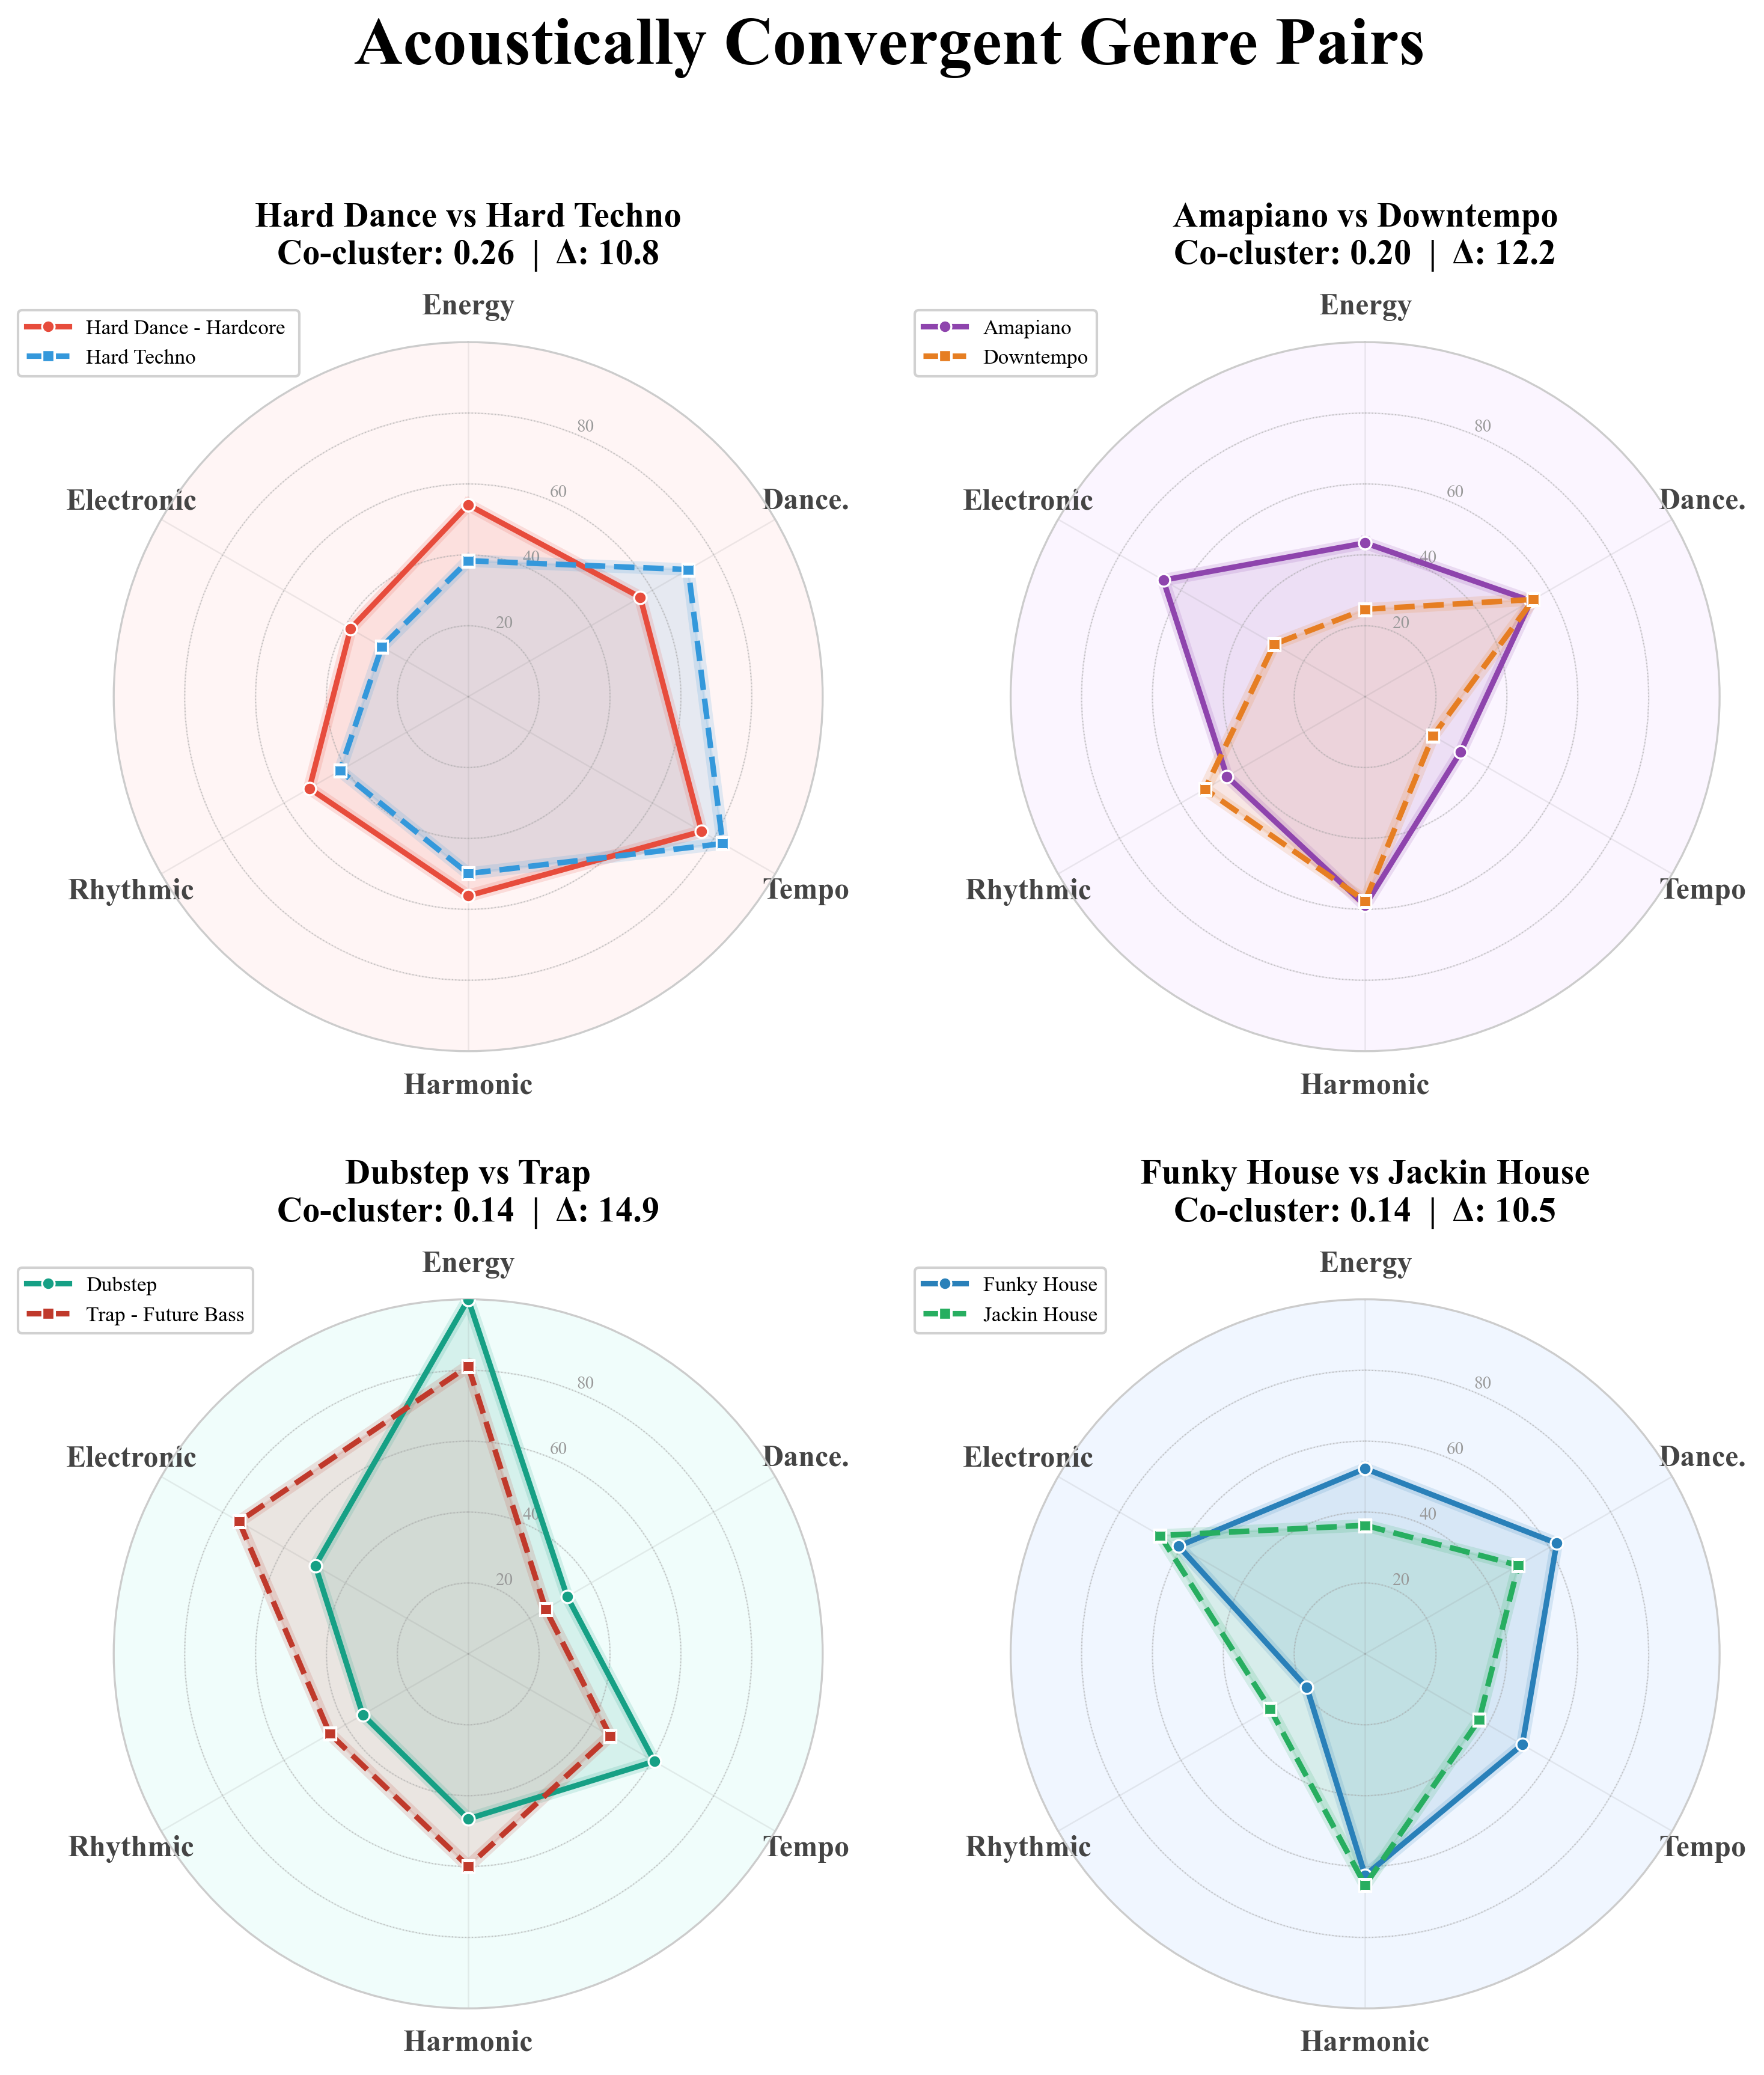
\includegraphics[width=0.95\columnwidth]{figs/paper/figa4_phantom_genre_profiles.png}
		\caption{Acoustically convergent ``phantom'' boundaries identified via dual filtering (high co-clustering frequency and mean profile difference $\Delta < 15$). Each subplot overlays the radar profiles of two commercially distinct genres possessing nearly identical acoustic signatures, illustrating explicit cases where commercial taxonomic boundaries lack concrete acoustic justification.}
		\label{fig:convergent}
	\end{figure}



\end{document}
